%%
%% This is file `sample-sigconf.tex',
%% generated with the docstrip utility.
%%
%% The original source files were:
%%
%% samples.dtx  (with options: `sigconf')
%% 
%% IMPORTANT NOTICE:
%% 
%% For the copyright see the source file.
%% 
%% Any modified versions of this file must be renamed
%% with new filenames distinct from sample-sigconf.tex.
%% 
%% For distribution of the original source see the terms
%% for copying and modification in the file samples.dtx.
%% 
%% This generated file may be distributed as long as the
%% original source files, as listed above, are part of the
%% same distribution. (The sources need not necessarily be
%% in the same archive or directory.)
%%
%% Commands for TeXCount
%TC:macro \cite [option:text,text]
%TC:macro \citep [option:text,text]
%TC:macro \citet [option:text,text]
%TC:envir table 0 1
%TC:envir table* 0 1
%TC:envir tabular [ignore] word
%TC:envir displaymath 0 word
%TC:envir math 0 word
%TC:envir comment 0 0
%%
%%
%% The first command in your LaTeX source must be the \documentclass command.
\documentclass[sigconf]{acmart}
\usepackage{multirow}
\usepackage{enumerate}
\usepackage{makecell}
\usepackage{bbm}
% \usepackage{paralist}
\usepackage{enumitem}
\usepackage{enumitem}
\usepackage{newtxtext,newtxmath}
\setlist{topsep=6pt, leftmargin=*}
%% NOTE that a single column version may be required for 
%% submission and peer review. This can be done by changing
%% the \doucmentclass[...]{acmart} in this template to 
%% \documentclass[manuscript,screen]{acmart}
%% 
%% To ensure 100% compatibility, please check the white list of
%% approved LaTeX packages to be used with the Master Article Template at
%% https://www.acm.org/publications/taps/whitelist-of-latex-packages 
%% before creating your document. The white list page provides 
%% information on how to submit additional LaTeX packages for 
%% review and adoption.
%% Fonts used in the template cannot be substituted; margin 
%% adjustments are not allowed.
%%
%%
%% \BibTeX command to typeset BibTeX logo in the docs
\AtBeginDocument{%
  \providecommand\BibTeX{{%
    \normalfont B\kern-0.5em{\scshape i\kern-0.25em b}\kern-0.8em\TeX}}}

%% Rights management information.  This information is sent to you
%% when you complete the rights form.  These commands have SAMPLE
%% values in them; it is your responsibility as an author to replace
%% the commands and values with those provided to you when you
%% complete the rights form.
\setcopyright{acmcopyright}
\copyrightyear{2023}
\acmYear{2023}
\acmDOI{XXXXXXX.XXXXXXX}

%% These commands are for a PROCEEDINGS abstract or paper.
\acmConference[Conference acronym 'XX]{Make sure to enter the correct
  conference title from your rights confirmation emai}{June 03--05,
  2018}{Woodstock, NY}
%
%  Uncomment \acmBooktitle if th title of the proceedings is different
%  from ``Proceedings of ...''!
%
%\acmBooktitle{Woodstock '18: ACM Symposium on Neural Gaze Detection,
%  June 03--05, 2018, Woodstock, NY} 
\acmPrice{15.00}
\acmISBN{978-1-4503-XXXX-X/18/06}

% \acmSubmissionID{661}

%%
%% Submission ID.
%% Use this when submitting an article to a sponsored event. You'll
%% receive a unique submission ID from the organizers
%% of the event, and this ID should be used as the parameter to this command.
%%\acmSubmissionID{123-A56-BU3}

%%
%% For managing citations, it is recommended to use bibliography
%% files in BibTeX format.
%%
%% You can then either use BibTeX with the ACM-Reference-Format style,
%% or BibLaTeX with the acmnumeric or acmauthoryear sytles, that include
%% support for advanced citation of software artefact from the
%% biblatex-software package, also separately available on CTAN.
%%
%% Look at the sample-*-biblatex.tex files for templates showcasing
%% the biblatex styles.
%%

%%
%% The majority of ACM publications use numbered citations and
%% references.  The command \citestyle{authoryear} switches to the
%% "author year" style.
%%
%% If you are preparing content for an event
%% sponsored by ACM SIGGRAPH, you must use the "author year" style of
%% citations and references.
%% Uncommenting
%% the next command will enable that style.
%%\citestyle{acmauthoryear}

%%
%% end of the preamble, start of the body of the document source.
% \usepackage{color}
\definecolor{green}{rgb}{0, 0.5, 0}
\definecolor{orange}{rgb}{0.8, 0.6, 0.2}
\definecolor{orange2}{rgb}{1.0, 0.6, 0.2}
\definecolor{red}{rgb}{1.0, 0.0, 0.0}
\definecolor{teal}{rgb}{0.0, 0.4, 0.4}
\definecolor{purple}{rgb}{0.65,0,0.65}
\definecolor{saffron}{rgb}{0.95,0.75,0.2}
\definecolor{turquoise}{rgb}{0.0,0.5,0.5}
\definecolor{black}{rgb}{0.0, 0.0, 0.0}
\definecolor{gray}{rgb}{0.5, 0.5, 0.5}


% \newcommand{\hang}[1]{{\color{orange}[Hang: #1]}}
% \newcommand{\hz}[1]{{\color{turquoise}#1}}%this is Hang too
% \newcommand{\ying}[1]{{\color{green}#1}}%this is Ying
% \newcommand{\cg}[1]{{\color{gray}#1}}

\newcommand{\hang}[1]{{\color{black}[Hang: #1]}}
\newcommand{\hz}[1]{{\color{black}#1}}%this is Hang too
\newcommand{\ying}[1]{{\color{black}#1}}%this is Ying
% \newcommand{\yingmodification}[1]{{\color{green}#1}}%this is Ying
% \newcommand{\redmarker}[1]{{\color{red}#1}}%this is Ying
\newcommand{\needattention}[1]{{\color{red}#1}}%this is Ying
\newcommand{\li}[1]{{\color{red}#1}}
\newcommand{\yingmodification}[1]{{\color{black}#1}}%this is Ying
\newcommand{\redmarker}[1]{{\color{black}#1}}%this is Ying
\newcommand{\cg}[1]{{\color{black}#1}}


\newcommand{\minor}[1]{{\color{black}#1}}
% \newcommand{\hang}[1]{{\color{purple}[Hang: #1]}}
% \newcommand{\hang}[1]{{\color{black}#1}}




% 
\usepackage{multirow}
\usepackage{booktabs}
\usepackage{subcaption}
\usepackage{amsmath,amsfonts,bm,amsthm,amssymb}
\usepackage{algorithm}
\usepackage{algorithmic}
\usepackage{graphics,graphicx,caption,float,color}
\usepackage{wrapfig}
\usepackage{bbm}
\usepackage{appendix}

% custom
\usepackage{listings}
\usepackage{xspace}
\newcommand{\tabincell}[2]{\begin{tabular}{@{}#1@{}}#2\end{tabular}} 
\usepackage{hhline}
\usepackage{multicol}
\usepackage{booktabs} 
\usepackage{makecell} % Xhline


% name of our model
\newcommand{\ffn}{TODO Our Method Name}
\newcommand{\ourabbr}{AdaptFormer\xspace}

\makeatletter
\newcommand*\bigcdot{\mathpalette\bigcdot@{.5}}
\newcommand*\bigcdot@[2]{\mathbin{\vcenter{\hbox{\scalebox{#2}{$\m@th#1\bullet$}}}}}
\makeatother

\definecolor{MyDarkBlue}{rgb}{0,0.08,1}
\definecolor{MyDarkGreen}{rgb}{0.02,0.6,0.02}
\definecolor{MyDarkRed}{rgb}{0.8,0.02,0.02}
\definecolor{MyDarkOrange}{rgb}{0.40,0.2,0.02}
\definecolor{MyPurple}{RGB}{111,0,255}
\definecolor{MyRed}{rgb}{1.0,0.0,0.0}
\definecolor{MyGold}{rgb}{0.75,0.6,0.12}
\definecolor{MyDarkgray}{rgb}{0.66, 0.66, 0.66}

\definecolor{Image}{RGB}{93,59,155}
\definecolor{Video}{RGB}{105,145,60}

\definecolor{ice}{RGB}{84,146,214}
\definecolor{fire}{RGB}{217,129,63}
\definecolor{baselinecolor}{gray}{.9}
\definecolor{poscolor}{RGB}{212,17,89}
\definecolor{negcolor}{RGB}{26,133,255}
\definecolor{bestcolor}{RGB}{238, 255, 238}
% copy-paste from Kaiming's MAE, used for ablation tables
\newcolumntype{x}[1]{>{\centering\arraybackslash}p{#1pt}}
\newcolumntype{y}[1]{>{\raggedright\arraybackslash}p{#1pt}}
\newcolumntype{z}[1]{>{\raggedleft\arraybackslash}p{#1pt}}
% \newcommand{\tablestyle}[2]{\setlength{\tabcolsep}{#1}\renewcommand{\arraystretch}{#2}\centering\footnotesize} % original style from MAE
\newcommand{\tablestyle}[2]{\setlength{\tabcolsep}{#1}\renewcommand{\arraystretch}{#2}\centering}%\footnotesize


\newcommand{\baseline}[1]{\cellcolor{baselinecolor}{#1}}
\newcommand{\bestcell}[1]{\cellcolor{bestcolor}{#1}}
\newcommand{\aaa}[1]{\textcolor{poscolor}{\small (#1)}}
\newcommand{\bbb}[1]{\textcolor{negcolor}{\small (#1)}}

\newcommand{\rebuttal}[1]{#1}
% \newcommand{\rebuttal}[1]{\textcolor{blue}{#1}}

\newcommand{\eg}{\emph{e.g.}}
\newcommand{\ie}{\emph{i.e.}}
\newcommand{\etal}{\emph{et.al.,}}


\begin{document}

%%
%% The "title" command has an optional parameter,
%% allowing the author to define a "short title" to be used in page headers.
\title{RetouchingFFHQ: A Large-scale Dataset for Fine-grained Face Retouching Detection}


%%
%% The "author" command and its associated commands are used to define
%% the authors and their affiliations.
%% Of note is the shared affiliation of the first two authors, and the
%% "authornote" and "authornotemark" commands
%% used to denote shared contribution to the research.
\author{Qichao Ying}
% \authornote{Both authors contributed equally to this research.}
\email{shinydotcom@163.com}
\affiliation{%
  \institution{Fudan University}
%   \streetaddress{2005 Songhu Rd}
  \city{Shanghai}
% %   \state{Ohio}
  \country{China}
%   \postcode{43017-6221}
}

% \orcid{1234-5678-9012}
\author{Jiaxin Liu}
\email{19307130299@fudan.edu.cn}
\affiliation{%
  \institution{Fudan University}
%   \streetaddress{2005 Songhu Rd}
  \city{Shanghai}
% %   \state{Ohio}
  \country{China}
}

\author{Sheng Li$^{\star}$}
% \authornote{Corresponding author.}

\email{lisheng@fudan.edu.cn}
\affiliation{%
  \institution{NVIDIA}
%   \streetaddress{5709 Shenjiang Rd}
  \city{Shanghai}
% %   \state{Ohio}
  \country{China}
}

\author{Haisheng Xu}
\email{hansonx@nvidia.com}
\affiliation{%
  \institution{NVIDIA}
%   \streetaddress{5709 Shenjiang Rd}
  \city{Shanghai}
% %   \state{Ohio}
  \country{China}
}

\author{Zhenxing Qian}
\authornote{Corresponding authors: Sheng Li and Zhenxing Qian.}

\email{zxqian@fudan.edu.cn}
\affiliation{%
  \institution{Fudan University}
%   \streetaddress{2005 Songhu Rd}
  \city{Shanghai}
% %   \state{Ohio}
  \country{China}
}

\author{Xinpeng Zhang}
\email{zhangxinpeng@fudan.edu.cn}
\affiliation{%
  \institution{Fudan University}
%   \streetaddress{2005 Songhu Rd}
  \city{Shanghai}
% %   \state{Ohio}
  \country{China}
}

\fancyhead{}
% \settopmatter{printacmref=false}

% \author{Anonymous ACM Multimedia Submission}

%%
%% By default, the full list of authors will be used in the page
%% headers. Often, this list is too long, and will overlap
%% other information printed in the page headers. This command allows
%% the author to define a more concise list
%% of authors' names for this purpose.
\renewcommand{\shortauthors}{Ying et al.}

% \newcommand{\tabincell}[2]{\begin{tabular}{@{}#1@{}}#2\end{tabular}} %放在导言区
%%
%% The abstract is a short summary of the work to be presented in the
%% article.
\begin{abstract}
The widespread use of face retouching filters on short-video platforms has raised concerns about the authenticity of digital appearances and the impact of deceptive advertising. To address these issues, there is a pressing need to develop advanced face retouching techniques. However, the lack of large-scale and fine-grained face retouching datasets has been a major obstacle to progress in this field. In this paper, we introduce RetouchingFFHQ
% ~\footnote{We will release the RetouchingFFHQ dataset after the anonymous reviewing stage.}
, a large-scale and fine-grained face retouching dataset that contains over half a million conditionally-retouched images. RetouchingFFHQ stands out from previous datasets due to its large scale, high quality, fine-grainedness, and customization. By including four typical types of face retouching operations and different retouching levels, we extend the binary face retouching detection into a fine-grained, multi-retouching type, and multi-retouching level estimation problem. Additionally, we propose a Multi-granularity Attention Module (MAM) as a plugin for CNN backbones for enhanced cross-scale representation learning. Extensive experiments using different baselines as well as our proposed method on RetouchingFFHQ show decent performance on face retouching detection. 
% With the proposed new dataset, we believe there is great potential for future work to tackle the challenging problem of real-world fine-grained face retouching detection.

%Extensive experiments show decent in-API and cross-API face retouching detection performance, therefore promoting more effective retouching regulation. More exampled images are attached in the supplementary material and the complete dataset will be made public for academic use after the anonymous reviewing stage.
\end{abstract}
%%
%% The code below is generated by the tool at http://dl.acm.org/ccs.cfm.
%% Please copy and paste the code instead of the example below.
%%
\begin{CCSXML}
<ccs2012>
 <concept>
  <concept_id>10010520.10010553.10010562</concept_id>
  <concept_desc>Computer systems organization~Embedded systems</concept_desc>
  <concept_significance>500</concept_significance>
 </concept>
 <concept>
  <concept_id>10010520.10010575.10010755</concept_id>
  <concept_desc>Computer systems organization~Redundancy</concept_desc>
  <concept_significance>300</concept_significance>
 </concept>
 <concept>
  <concept_id>10010520.10010553.10010554</concept_id>
  <concept_desc>Computer systems organization~Robotics</concept_desc>
  <concept_significance>100</concept_significance>
 </concept>
 <concept>
  <concept_id>10003033.10003083.10003095</concept_id>
  <concept_desc>Networks~Network reliability</concept_desc>
  <concept_significance>100</concept_significance>
 </concept>
</ccs2012>
\end{CCSXML}

\ccsdesc[500]{Computing methodologies ~ Artificial intelligence; Computer vision; Neural networks}
\keywords{Datasets; Deep Learning; Face Retouching Detection}


%% A "teaser" image appears between the author and affiliation
%% information and the body of the document, and typically spans the
%% page.
\begin{teaserfigure}
  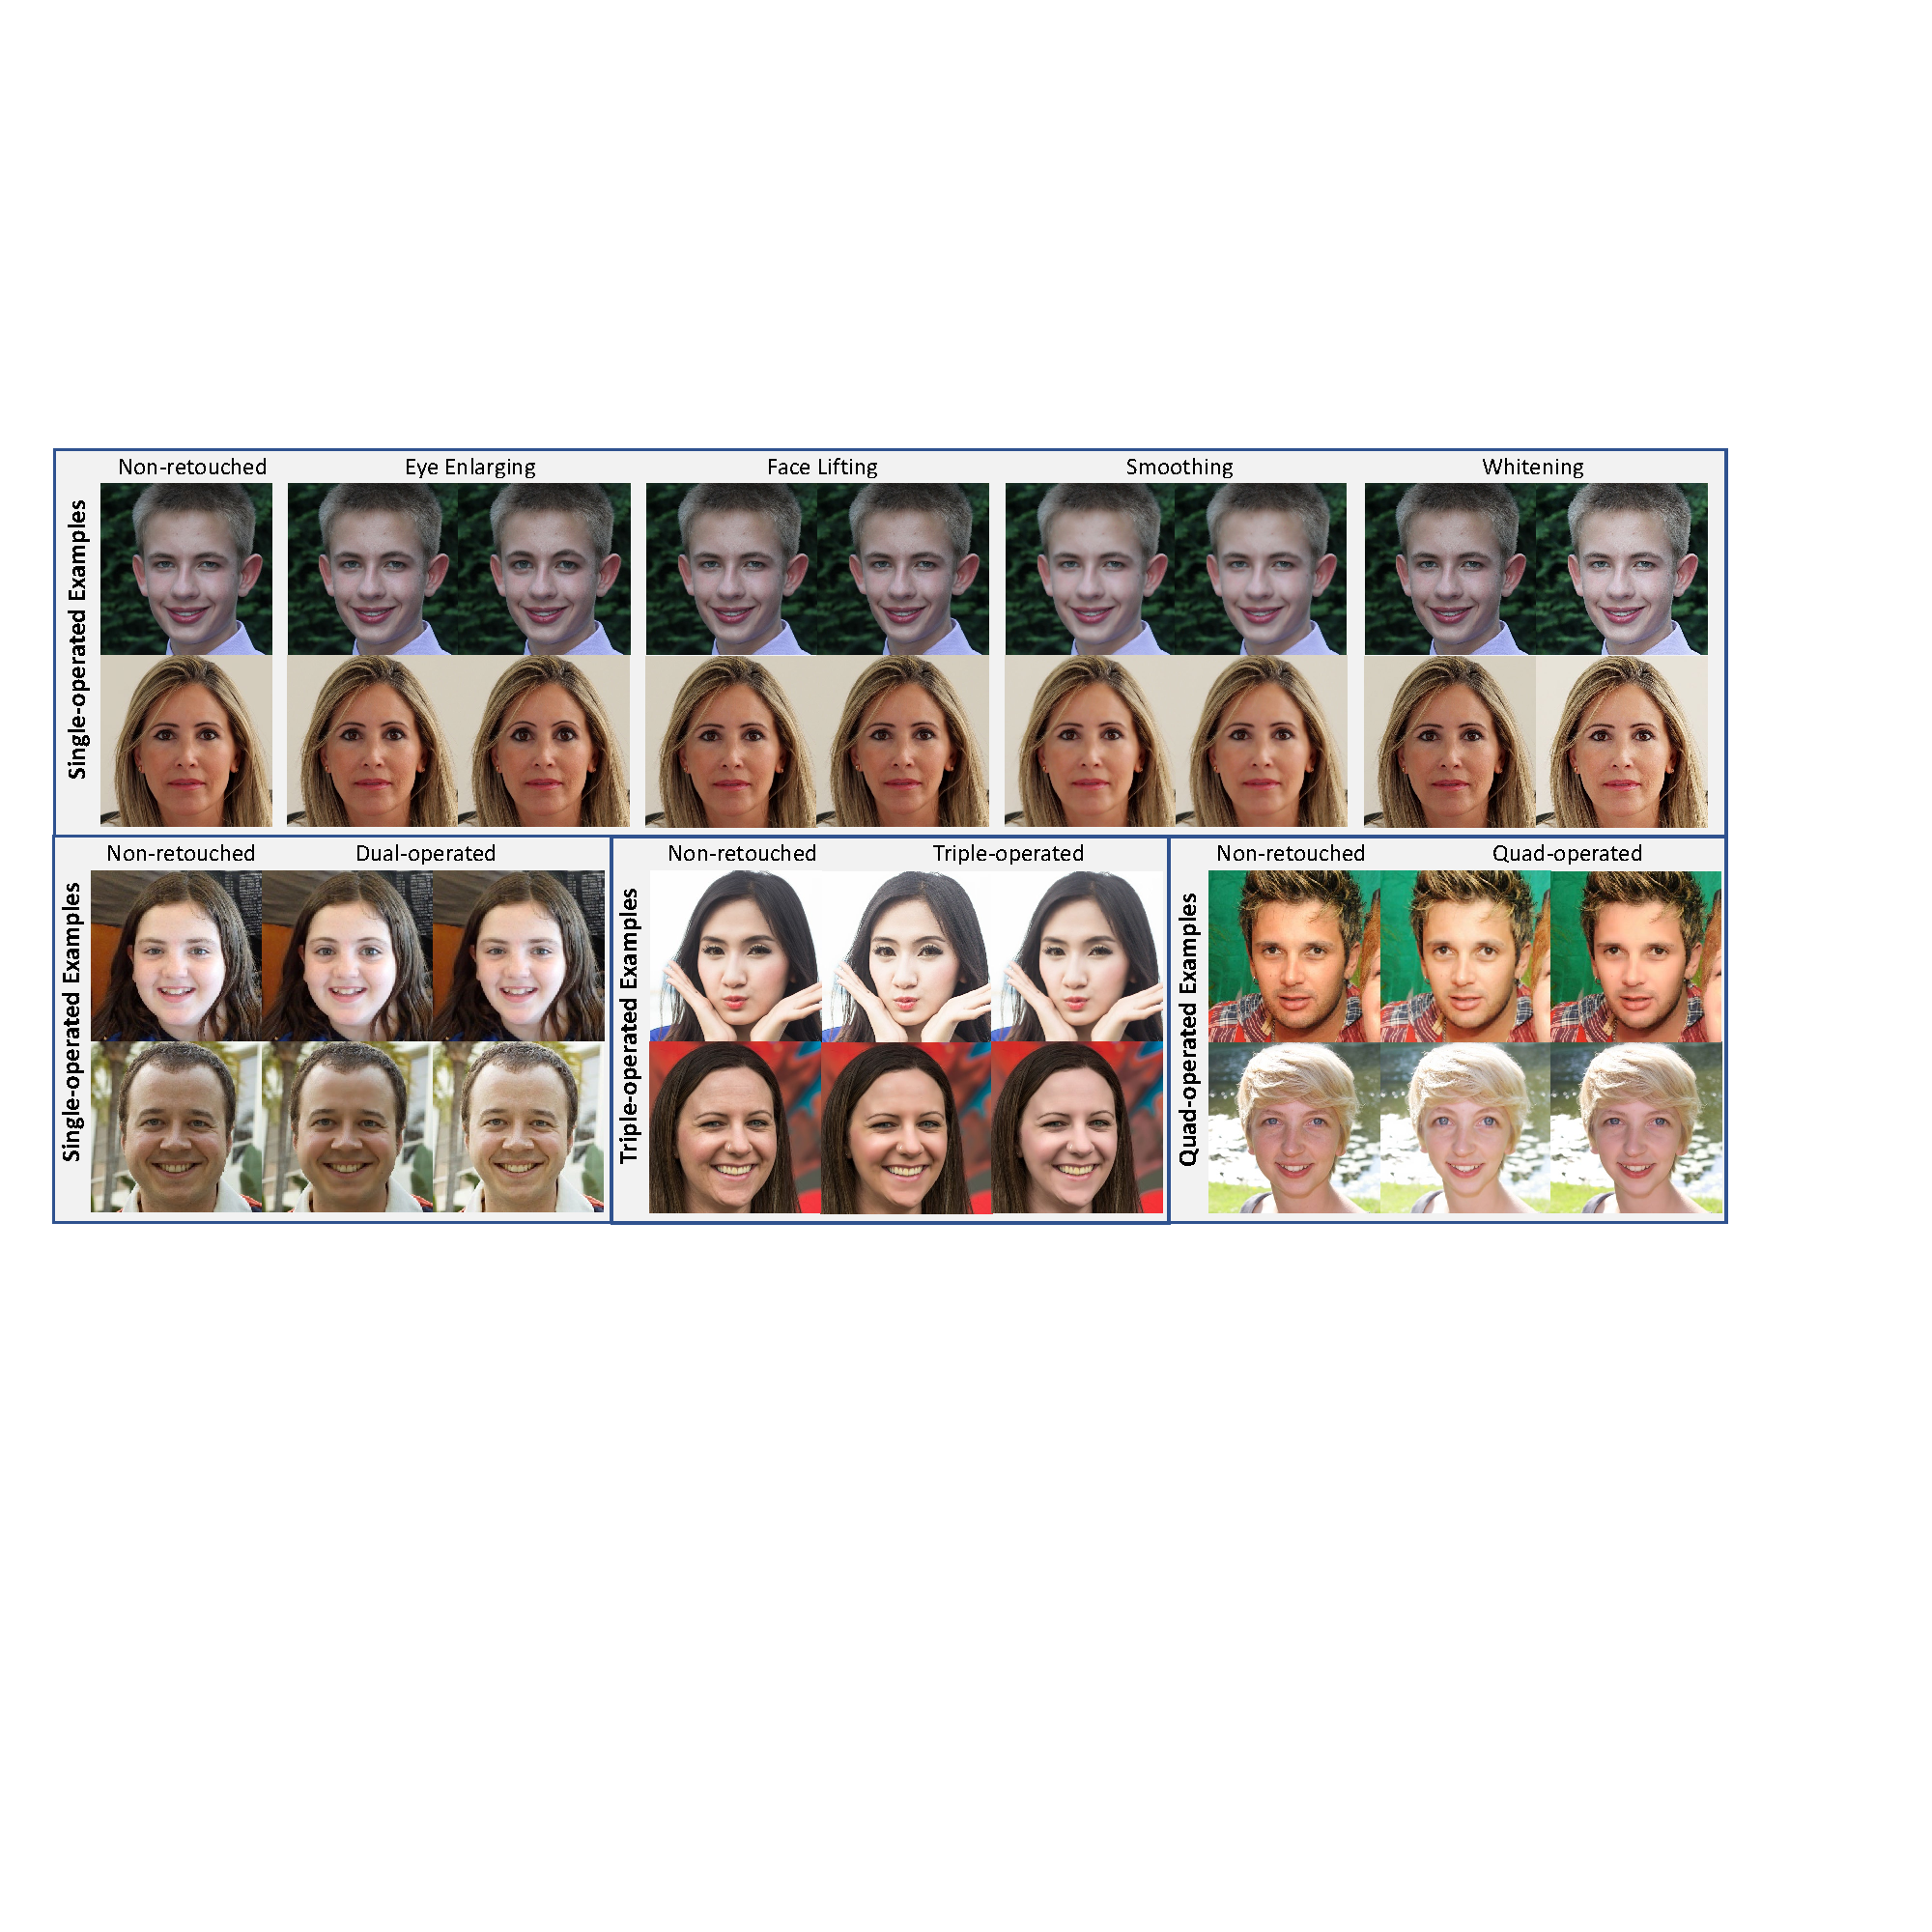
\includegraphics[width=\textwidth]{figures/more_examples.pdf}
  \caption{Examples of RetouchingFFHQ, a fine-grained face retouching dataset containing over half a million images. (Upper) Examples of single-operated images. In each operation group, the magnitude of the left / right images are respectively 30 / 90. (Lower) Examples of dual-operated to quad-operated images where the annotations are omitted for better visualization.}
  % \Description{Enjoying the baseball game from the third-base
  % seats. Ichiro Suzuki preparing to bat.}
  \label{fig:teaser}
\end{teaserfigure}

% \received{20 February 2007}
% \received[revised]{12 March 2009}
% \received[accepted]{5 June 2009}

%%
%% This command processes the author and affiliation and title
%% information and builds the first part of the formatted document.
\maketitle

\section{Introduction}
The increasing popularity of short-video platforms such as TikTok, YouTube Shorts, and Facebook Reels has led to a surge in the use of face retouching filters~\cite{rathgeb2022handbook}. 
With just a click, users can achieve a more glamorous and visually striking appearance, thanks to a range of retouching functions such as face lifting, eye enlargement, whitening, and smoothing. 
While many people use these filters moderately and innocently, some go to the extreme to completely alter their appearance to deceive their audience for commercial purposes, e.g., news where people got scammed in online romance due to retouched appearance.
% This raises concerns about the authenticity of digital appearances as well as the impact of deceptive advertising, particularly in the cosmetic industry, which may use retouched images to exaggerate the effects of aesthetic medicine. Besides, studies have been conducted to unveil that heavy face retouching would seriously jeopardize the security of face recognition systems  ~\cite{bharati2016detecting,rathgeb2019impact,VMUYMU}. 
% It is necessary and important to identify the existence of retouching from the face images.   

%Digitally altered face images can also have a negative psychological impact on viewers' self-esteem, particularly among young people, by promoting wrong beauty standards.
%
% In Norway, the term "kroppspress" is popularly used to criticize advertisers and influencers for creating "impossible perfect illusions" that lead young people to pursue unrealistic beauty standards.

Currently, there are three main strategies to address the aforementioned issue. The first is \textbf{visible watermarking by law enforcement}.
For instance, the Norwegian government~\cite{Norwaylaw} 
% ~\footnote{\url{https://www.insider.com/norway-law-social-media-influencers-advertisers-disclose-edited-images-2021-7}}. 
has mandated that all ads featuring modified body shapes and facial appearances must be labeled with a visible disclaimer which takes up at least 7\% of the whole image. 
The United States, Israel and Germant also have similar labeling requirements~\cite{USlaw,Israellaw}.
% ~\footnote{\url{https://www.congress.gov/bill/113thcongress/house-bill/4341}}
% France, Canada, Germany and Australia 
The visible watermarks severely reduce the image quality, and it can deter users even from mild use of face retouching.
The second is \textbf{invisible watermarking}, which imperceptibly embeds fragile watermarks into the face images ~\cite{ying2021image,asnani2022proactive,he2020semi}. The watermarks will be damaged once the face images are retouched. This kind of approaches requires people to proactively embed the watermark into the face images once captured.
% , which may not be practical in real world applications.   
The third is \textbf{face image retouching detection} to determine whether the face images are retouched without any proactive processes. Face image retouching detection is a challenging problem as the retouching may only mildly change the image content. Directly applying the face manipulation (also DeepFake) detection~\cite{jain2018detecting,jain2020detecting} or image manipulation detection~\cite{MVSS,mantra} schemes would not be appropriate to tackle such a challenge. Be aware of this, researchers have devoted efforts to schemes which are developed specifically for face image retouching detection~\cite{wang2020deep,rathgeb2020differential}.  
%However, the face retouching 

%There are also schemes proposed specifically for face retouching detection, 
% \begin{figure}[!t]
% 	\centering
%     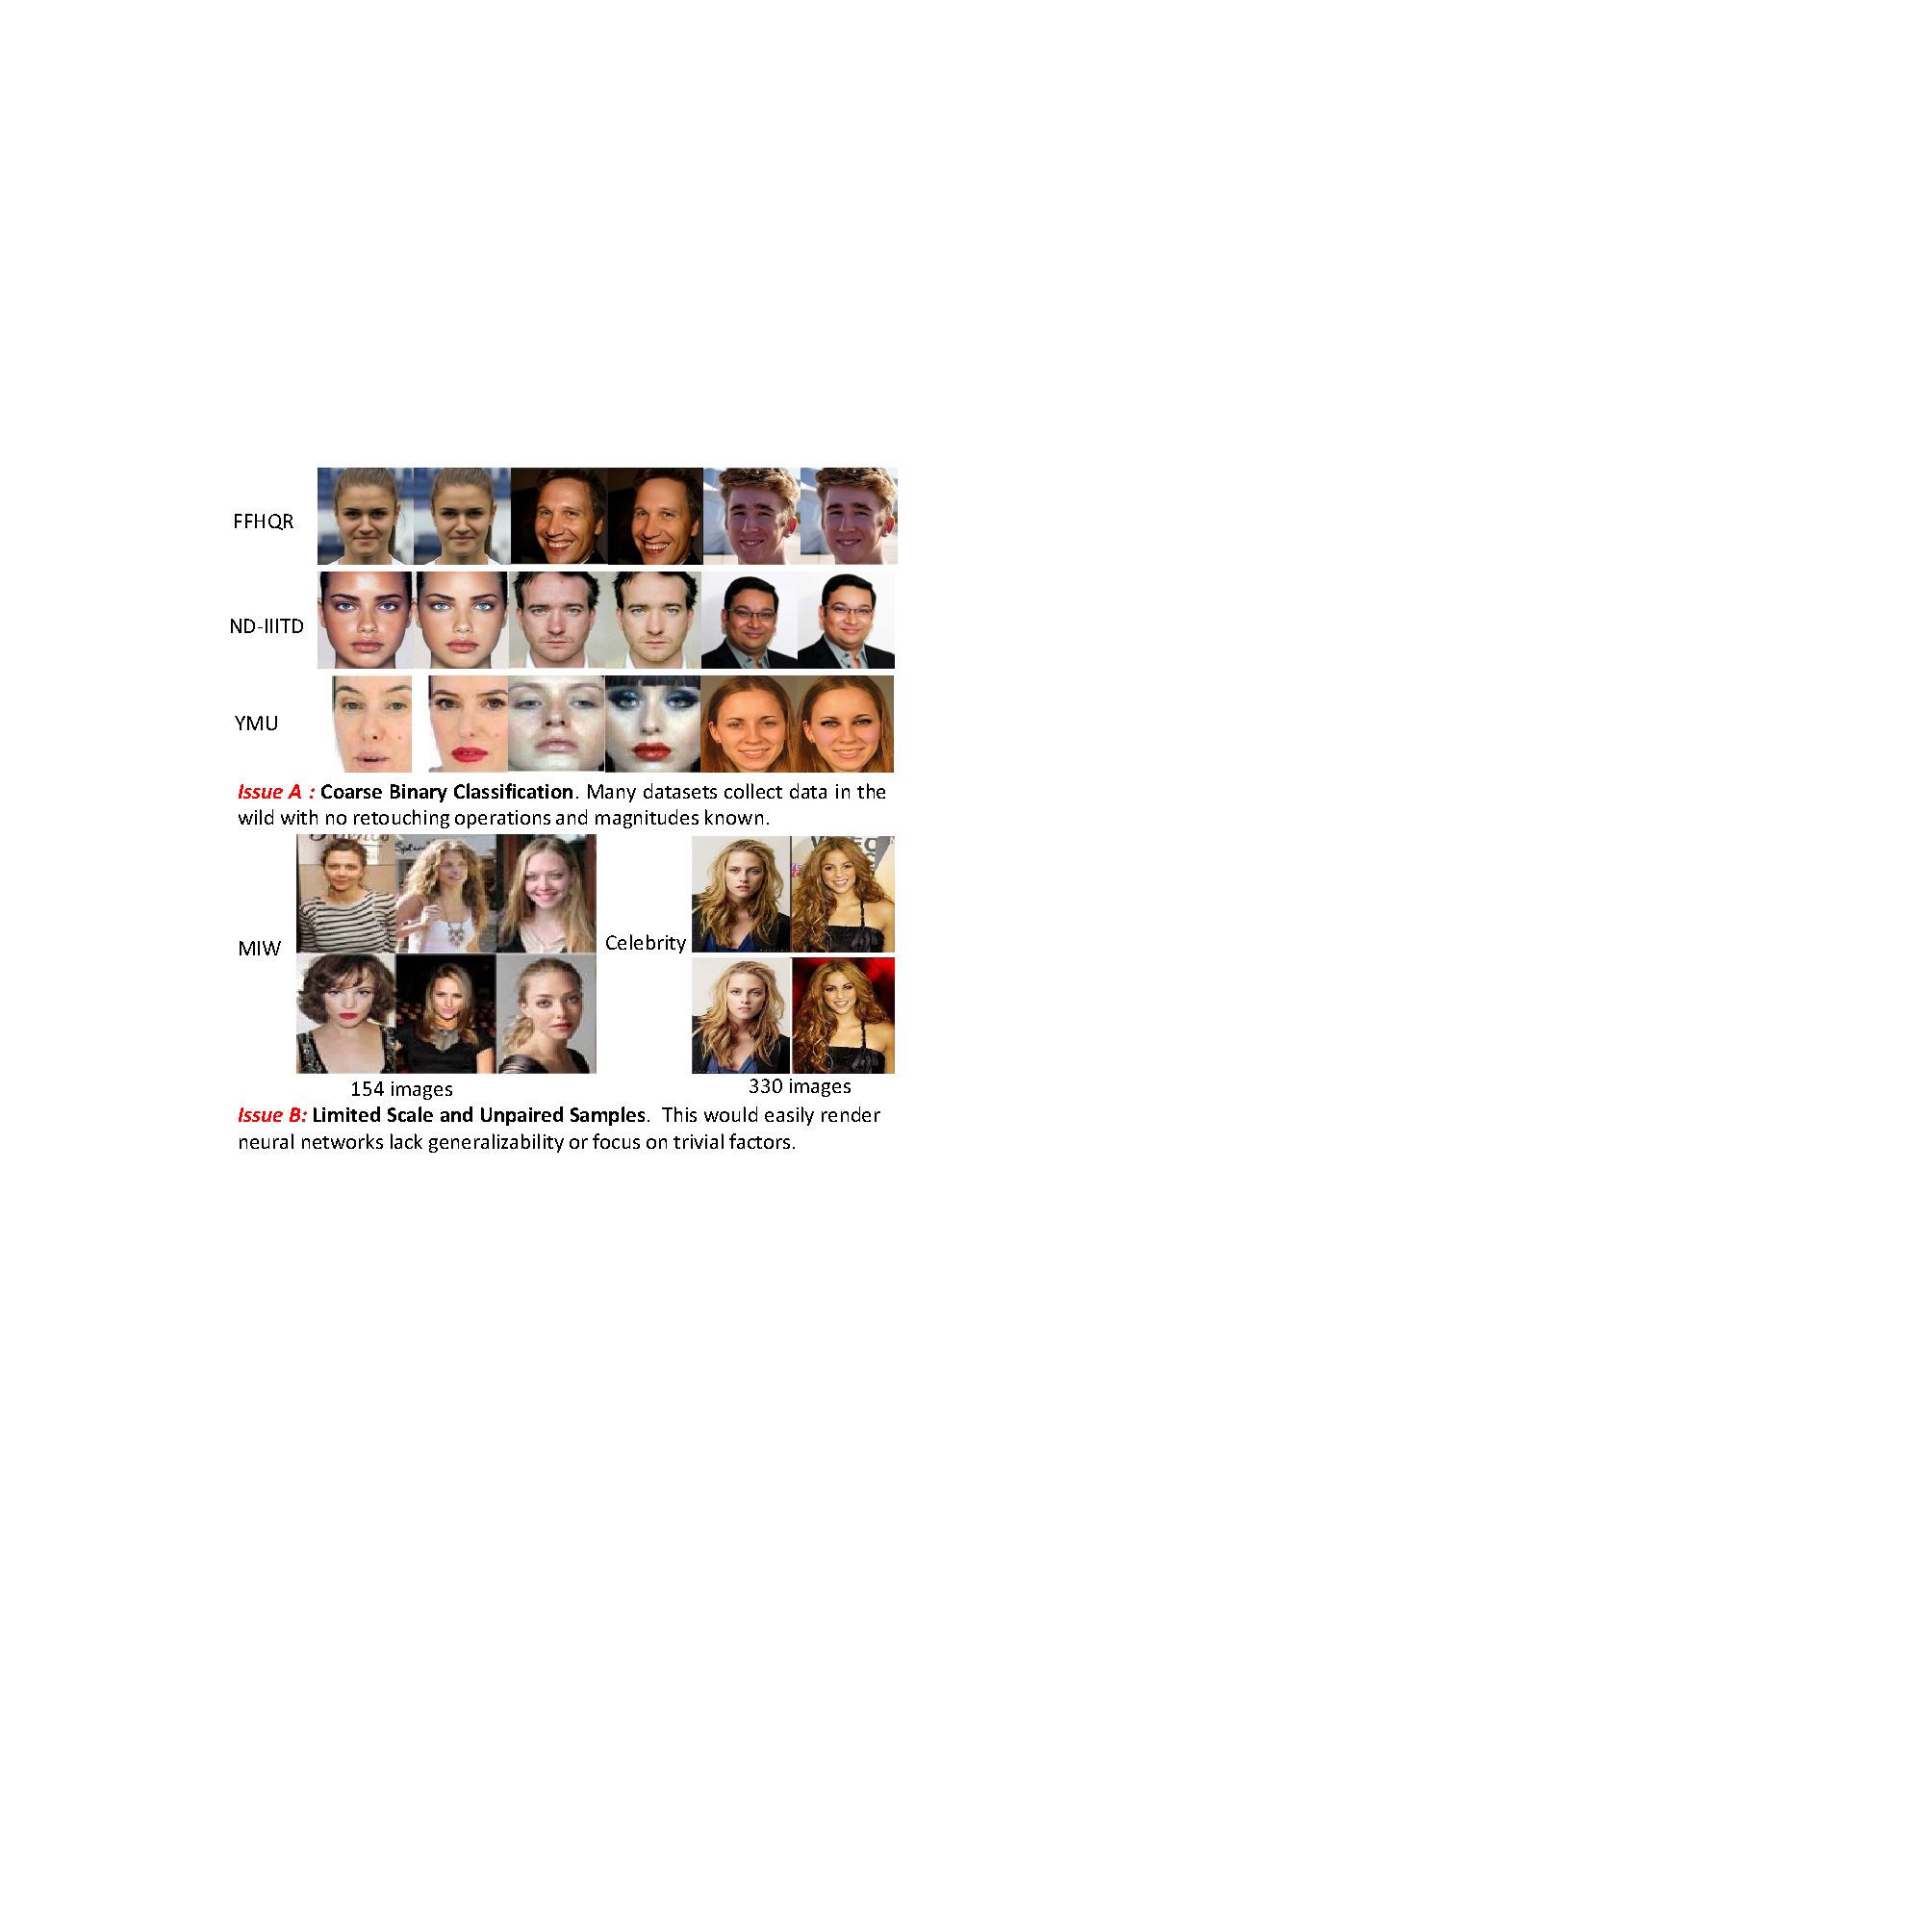
\includegraphics[width=0.48\textwidth]{figures/related_datasets.pdf}
% 	\caption{Existing issues of the closely-related datasets. We invite readers to compare them with the examples in Fig.1.}
% 	\label{fig:dataset_comparison}
% \end{figure}

\begin{table*}
% \renewcommand\arraystretch{1.15}
\begin{center}
   \caption{A summary of existing datasets related to face retouching. RetouchingFFHQ is the largest and the first fine-grained dataset for face retouching consisting of 500k images processed by commercial APIs. $S$, $W$, $E$, $L$ respectively denote skin-smoothing, face-whitening, eye-enlarging and face-lifting.}
   \label{tab:dataset_compare}
\begin{tabular}{c|c|c|c|c|c}
\hline 
\multirow{2}{*}{Datasets} & \multicolumn{2}{c|}{Shots} & \multicolumn{2}{c|}{Image Attributes} & \multirow{2}{*}{Remarks}\\
\cline{2-5}
&  \#Ori. & \#Retou. & Operation & Level&\\
\hline
\hline
Kee et al.\cite{kee2011perceptual} & 468 & 468 & 1 (No distinction) & 5 (subjective) & \ying{Images crawed from the Internet}\\
\hline
YMU\cite{VMUYMU} & 151 & 300 & 1 (No distinction) & on / off  & Images of Caucasian females\\
\hline
VWU\cite{VMUYMU} & 51 & 153 & 3 (eyemakeup / lipstick / both) & on / off & Images of Caucasian females\\
% \hline
% MIW\cite{MIW} & 77 & 77 & 154 & 1 (No distinction) & on / off & \ying{Images crawed from the Internet}\\
\hline
Celebrity\cite{bharati2016detecting} & 165 & 165 & 1 (No distinction) & on / off & \ying{Images crawed from the Internet}\\
\hline
ND-IIITD\cite{bharati2016detecting} & 325 & 2275 & 7 (hybrid presets) & on / off & Using Portrait-pro Studio Max\\
\hline 
MDRF\cite{bharati2017demography} & 600 & 2400 & 2 (App type) & on / off & Using BeautyPlus/Potrait Pro\\
\hline
Rathgeb et al.\cite{rathgeb2020prnu} & 100 & 800 & 5 (hybrid filters) & on / off & Using five Apps with hybrid retouching\\
\hline
DiffRetouch\cite{rathgeb2020differential} & 1726 & 9078 & 7 (hybrid filters) & on / off & Improved version of Rathgeb et al.\cite{rathgeb2020prnu}\\
\hline
BeautyGAN~\cite{li2018beautygan} & 1115 & 2719 & 1 (No distinction) & on / off & GAN-based style-transfer with references\\
\hline
FFHQR\cite{shafaei2021autoretouch} & 70000 & 70000 & 1 (No distinction) & on / off & Hybridly retouched by professional editors \\
\hline
\hline
\textbf{RetouchingFFHQ} & 58158 & 652568 & \makecell{Single-operated ($S$, $W$, $E$, $L$)\\Dual-operated ($S+W$, etc.)\\Triple-operated ($S+W+E$, etc.)\\Quad-operated ($S+W+E+L$)} & \makecell{$S: 0/30/60/90$\\$W: 0/30/60/90$\\$E: 0/30/60/90$\\$L: 0/30/60/90$} & \makecell{Controllably Generated using Commercial\\APIs: Megvii, Alibaba and Tencent}\\
\hline 
\hline
\end{tabular}
\end{center}
\end{table*}

In literature, many datasets have been constructed for the task of face retouching detection, as summarized  in Table 1. 
Despite the progress, there are still several challenges that need to be addressed.
Firstly, the existing datasets are limited in size, with the largest one, i.e., FFHQR~\cite{shafaei2021autoretouch}, containing 70k retouched images, and the rest containing fewer than 10k samples.
Consequently, these datasets may not be sufficient to train robust detection networks.
Secondly, the current datasets lack fine-grained annotations of retouching types and levels.
For instance, some datasets, such as VWU~\cite{VMUYMU}, only contain images of Caucasian females with a limited range of retouching types. 
Other datasets, such as ND-IIITD~\cite{bharati2016detecting}, Rathgeb et al.\cite{rathgeb2019impact}, and DiffRetouch\cite{rathgeb2020differential}, employ binary classification for retouching detection, ignoring the diverse types and degrees of retouching. Kee et al.~\cite{kee2011perceptual} categorize the retouching levels, but still mix retouched images of various types. We believe that binary classification may not sufficient to capture the complexity of face retouching, which can range from innocuous cosmetic enhancement to malicious forgery. Therefore, there is a need to build more fine-grained face retouching datasets which can be used to train classifiers to capture the diverse types and levels of retouching.

%First of all, seven out of ten listed datasets are with less than 1000 samples and therefore not large enough to train a well-rounded detection network.
%Second, eight of them are in binary-classification style, which blindly account for a wide range of retouched images into a unified class.
%On one hand, while severe retouching behavious are malicious and should be banned once detected, mild ones can be benign and acceptable.
%On the other hand, even though some retouched images do not affect face recognition systems, they should also be figured out if retouching is prohibited by law.
%From this view, the existing works largely cannot reason beyond \textit{real} and \textit{fake},
% , lack fine-grained supervision to discover clues among different types and levels of retouching, 
%and therefore leave little room for \textit{customization} in retouching regulation.
% of each retouching behavior (mainly according to the levels).
% For example, how to distinguish mild and benign retouching from those heavy and fraudulent ones? 
% Overall, we believe that face retouching detection is less historically investigated compared to its close-related neighbors, e.g., DeepFake detection~\cite{li2020face,zhang2022patch}, and 
%We believe the utmost issue is the lack of large-scale and fine-grained face retouching datasets.
%With the rising of short-video platforms such as TikTok, Youtube Short and Facebook Reels, the abuse of face face retouching or face retouching has become a common trend on the social media, and even identification cards are not strictly enforced to be bare face. Our work is motivated by short video live streaming such as TikTok, which is one of the biggest trends on social media right now, with users all over the world. In this field, face retouching is likely the potential rule while un-retouched photos are an exception.

%Face face retouching can be either make-up or digital editing, and the aim is to make the face look more beautiful or appealing due to the fascination toward a few factors such as fair complexion and flawless skin. With the availability of easy-to-use image editing tools, beautifying an image is a very simple operation and can be widely used by almost everyone. 

%While the majority of these images are created for well-intention, they may be used with malicious intent for negative applications or causing social problem invisibly. In the cosmetic industry, it can be used for deceptive advertising to show the effects of aesthetic medicine. Digitally retouched images can negatively affect the self-esteem of the viewers by trying to follow the societal norm of pleasant appearance, which also leads to body dissatisfaction amongst people, especially for youngsters and gives rise to various psychological diseases. Besides, face recognition accuracy can be greatly reduced when the probe image and the enrolled image are using different types and degree of face retouching. 
% To deal with these problems, some countries such as Israel, UK, and USA have enacted laws to regulate the use of retouched images. In order to strictly abide by these laws and to reduce the potential problems, the successful detection of digitally retouched images is a promising countermeasure. In order to train an effective detector, a large amount of both unaltered and retouched images are required. This derives the existing datasets such as YMU, MIW and Celebrity. The most commonly used dataset is called ND-IIITD, which contains thousands of images with binary labels. 

% All of these schemes have some common drawbacks. Firstly, existing algorithms are mostly considered binary classification problems, \ying{whereas} in real-world scenarios, the category and extent of image face retouching are also important since the mild face retouching may be harmless while severe retouching may be potentially malicious. 
% \ying{Secondly, the existing datasets are either not large in quantity, e.g., less than one thousand images, or consist of untraceable images and blind retouching}. 
% Though it can also adjust the higher level semantics of the images, the dataset is still developed for binary classification where the specific retouching are not recorded.
% In summary, it still needs a more adequate dataset to extend existing problems and consider further detection classification.

% We identify potential weaknesses in existing beauty detection data sets. Firstly, they all have too few images. Currently, the widely used datasets contain a minimum of 154 images (MIW) and a maximum of 4,875 images (ND-IIITD), among which the number of individuals is mostly hundreds. Compared with other mainstream image classification tasks at present, the data amount is small. Secondly, the composition of personnel in the datasets is also relatively simple, so it is difficult to cover all factors such as different ages and races, which is not completely consistent with the real situation and demand. The generalization ability of the model is limited. Besides, the binary labels can not reflect the real situation, in which the type and degree of beauty is equally important to the actual problem. We not only need to know whether the image has been retouched, but also to know how much the image has been modified. Simple modification is harmless, while excessive packaging may hide evil intentions. Most of the existing data sets only annotate whether the image is processed or not. There are also some data sets that use manual annotation to mark the degree of image processing, with stronger subjective factors and the influence of individual aesthetic differences.

% \noindent\textbf{Our Large-Scale Fine-Grained Face Retouching Dataset.} 
To overcome the limitations of existing datasets, we construct a large-scale fine-grained face retouching dataset (RetouchingFFHQ) in this paper, which consists of over half a million retouched face images with a range of different retouching types and levels. Our dataset is constructed based on the well-known FFHQ dataset~\cite{FFHQ}, where different face retouching operations are performed on these images in terms of specific types and levels. To generate the retouched images, we utilize three popular commercial online APIs including Megvii~\cite{Megvii}, Tencent~\cite{Tencent}, and Alibaba~\cite{Alibaba}. Each retouched image in our dataset includes one to four types of retouching, namely, eye-enlarging, face lifting, skin smoothing, and face whitening, which are the most commonly used geometric and non-geometric operations on social media platforms. To ensure fine-grained annotations, we have categorized the levels of each retouching into four classes: off (0), slight (30), medium (60), and heavy (90). Figure 1 provides some examples, with more provided in the supplementary material.
The complete dataset will be made public for academic use after the anonymous reviewing stage.

Overall, the advantages of our dataset are listed below.

\begin{itemize}
\item \textbf{Large-Scality and High Quality}. 
RetouchingFFHQ is the largest face retouching dataset to date, consisting of 652,568 retouched images and 58,158 non-retouched images. To ensure high quality, we conducted strict data cleaning to exclude face images that might not be used in real-world face retouching applications, e.g., \textit{closed eyes}, \textit{poor lighting conditions}, \textit{incomplete faces}, etc.

\item \textbf{Fine-grained labeling.} RetouchingFFHQ extends the previous binary classification problem of face retouching detection into a fine-grained multi-label fashion. RetouchingFFHQ enables the detection of multiple types of retouching and their corresponding levels, providing a more nuanced understanding of the types and extent of face retouching in social media platforms.

%\item \textbf{Customization}. 
%We introduce three task-specific performance indicators that help users select models according to their requirements, including the true positives, false negatives, and the overall accuracy. These indicators allow users to tailor the model's performance to their specific use case, ensuring that it meets their individual needs.
%Besides, users can customize the blockage of excessively retouched images in the real world thanks to the multi-labeled predictions.

\item \textbf{Cross APIs}. RetouchingFFHQ is composed of retouched images made by three commercial APIs. Users can evaluate the performance of the detection models using both in-API (training and testing based on the same API) and cross-API (training and testing based on different API) settings.
\end{itemize}

In addition to the dataset, we propose a novel Multi-granularity Attention Module (MAM) that can refine hierarchical representations and compare information from different receptive fields to improve the detection performance. Extensive experiments demonstrate that, with the proposed MAM as a plugin, the baselines can gain remarkable performance gain for face retouching detection.
% We expect further works to utilize the new dataset to further tackle the problem of fine-grained face retouching detection.
With the proposed new dataset, we believe there is great potential for future work to tackle the challenging problem of real-world fine-grained face retouching detection.

%identified a challenge with existing CNN network architectures in effectively modeling the multi-granularity relationships between hierarchical deep representations for face retouching detection. To address this challenge, we propose a novel Multi-granularity Attention Module (MAM) that can refine hierarchical representations and compare information from different receptive fields to improve detection performance. 
%We build a number of Transformer-based, CNN-based and hybrid baseline networks and measure their performance in view of both in-API and cross-API detection.


% We first introduce RetouchingFFHQ in Section 2, and then propose MAM for enhanced fine-grained face retouching detection in Section 3.
% Section 4 presents and discusses the experimental results.
% Having elaborated the dataset, we introduce related works and datasets of face retouching in Section 5 and compare them with RetouchingFFHQ.
% Finally, we conclude the paper in Section 6.

% \begin{figure*}[ht]
% 	\centering
% 	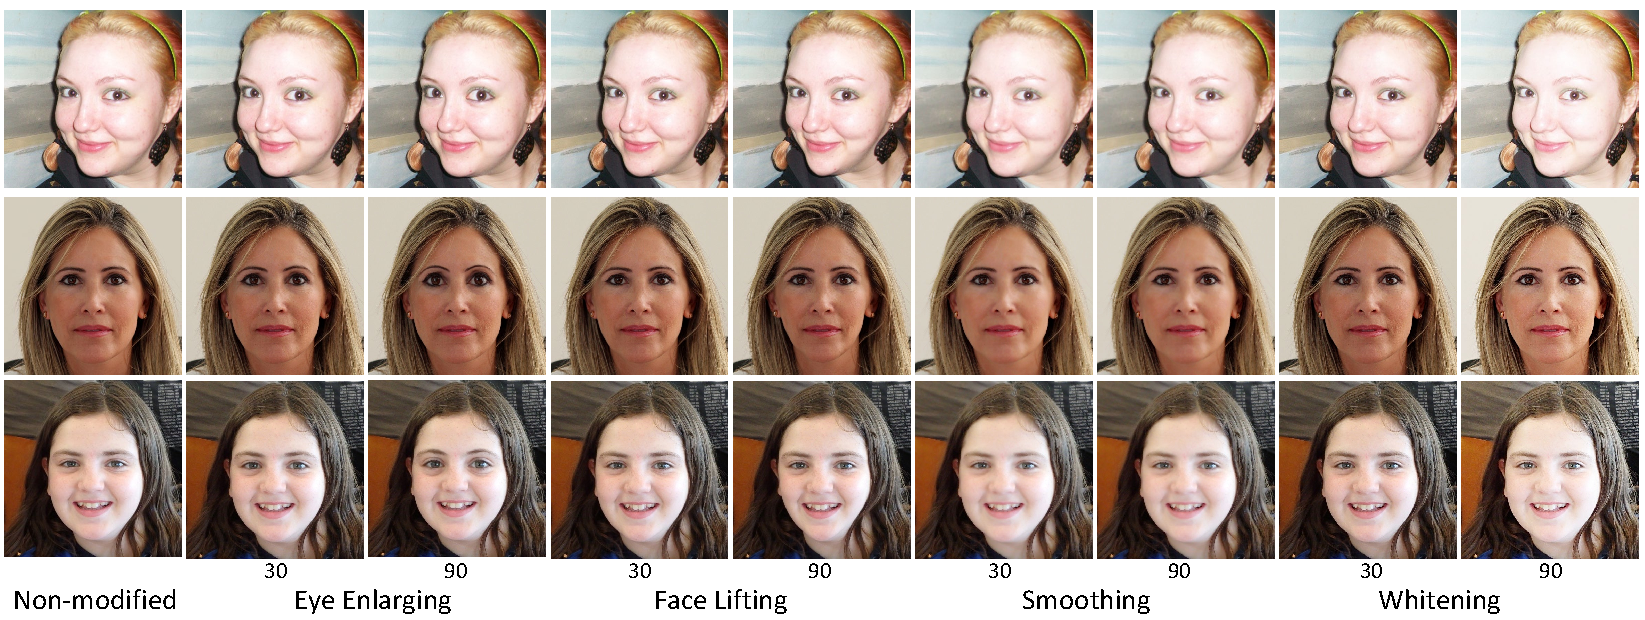
\includegraphics[width=1.0\textwidth]{figures/example_one.pdf}
% 	\caption{Examples of retouched images. For many pairs of images, the differences might be trivial yet resulting in more appealing appearances. Better zoom in for details.}
% 	\label{fig_example_one}
% \end{figure*}

\section{Related Works}
% \subsection{Existing Face Retouching Datasets} 
% \noindent\textbf{face Retouching Generation and Detection.} 
Table~\ref{tab:dataset_compare} summarizes the existing datasets related to face retouching.
Specifically, 
Kee et al.~\cite{kee2011perceptual} develop a dataset with 436 retouched images and invite volunteers to rank the amount of photo alteration on a scale of one to five.  
% subjective metric where images are rated on the degree to which they have been digitally altered by  estimating geometric and photometric changes. 
% propose a metric for assessing the perceptual effects of face retouching on human observers, which is widely used in the literature. 
YMU and VMU~\cite{VMUYMU} are two compact datasets proposed to determine the presence of makeup operations from their impacts on automated face recognition.
% To explore the impact of makeup or retouching on the performance of face recognition algorithms, several small datasets, such as YMU, VMU\cite{VMUYMU}, and MIW\cite{MIW}, are constructed.
Then, Bharati et al.\cite{bharati2016detecting} introduce two larger datasets, namely, ND-IIITD and Celebrity.
The ND-IIITD dataset contains seven presets, each containing eight to twelve different types of retouching. 
% and accordingly propose supervised deep Boltzmann machine algorithm is proposed to learn discriminative features from the retouched images. 
In~\cite{bharati2017demography}, Bharati et al further propose Multi-Demographic Retouched Faces (MDRF) to investigate the effect of demography and gender on the accuracy of retouching detection.
Rathgeb et al.\cite{rathgeb2020prnu} conduct qualitative assessment over beautification apps and five are chosen to create a new dataset. 
The photo response non-uniformity (PRNU) is used for retouching detection.
DiffRetouch~\cite{rathgeb2020differential} use seven apps, such as \textit{AirBrush} and \textit{BeautyPlus}, to generate nearly 10k hybrid retouched images, with each app showing different characteristics.
Apart from collecting data from apps, some recent methods also utilize GAN-based technologies to create new face retouching datasets.
BeautyGAN~\cite{li2018beautygan} build up a make-up dataset using style-transfer, which can achieve virtual makeup tryout.
Shafaei et al. propose FFHQR~\cite{shafaei2021autoretouch} which contains 70k retouched images by professional editors and is designed for automatic face retouching. 
% There are other generative models that could perform comprehensive digital retouching~\cite{jiang2020psgan,chen2019beautyglow}.
Besides, some tailored detection networks~\cite{jain2018detecting,jain2020detecting,geng2020masked} are proposed for these datasets.

% Jain et al.\cite{jain2018detecting,jain2020detecting} propose a hierarchical approach called DAD-HCNN for detecting both retouching and GAN-generated images, achieving high accuracy on the ND-IIITD dataset.
% Besides these datasets, there are also other facial alteration or beautifying algotirhms using GANs~\cite{wang2021towards,}, but these methods are mostly 
% However, this dataset only provides binary labels, and the processing methods used are disparate. While these datasets are valuable resources for research in face retouching, our study seeks to address limitations in existing datasets by providing a larger and more diverse dataset with fine-grained labels and standardized processing methods.

These datasets and detection networks are valuable and promote the development of the literature.
But there still exist issues regarding the binary-classification restriction and the limitation in dataset scale.
% less existing datasets and forensics works address the robustness issue in face retouching detection~\cite{rathgeb2021effects}, which is critical in that
% real-world face retouching are favored by popular online short-video platforms such as TikTok or Youtube Short, which normally compress livestream videos for transmission.
% deep networks trained on uncompressed images can be easily susceptible to trivial distortions~\cite{robust1,robust2}. 
% , e.g., fragile traces such as PRNU might not work.
We attempt to address them via RetouchingFFHQ.

\begin{table*}
% \renewcommand\arraystretch{1.15}
\begin{center}
   \caption{A Summary of RetouchingFFHQ, which contains three subsets with images retouched by different APIs.}
   \label{tab:dataset_summary}
\begin{tabular}{c|c|c|c|c|c}
\hline 
Image Kind & Available APIs & \#Retouched per sample & \#Num Retouched & \#Retouched/person & Avg. PSNR\\
% \multirow{3}{*}{Supervised pretraining}
\hline
\hline
Subset-0: Non-retouched& / &/&58158&/&/\\
\hline
\multirow{3}{*}{Subset-1: Single-operated}& Megvii &1 per \{sample, type\}&66940&4&29.33\\
% &\multirow{3}{*}{\makecell{Smoothed,\\Eye-enlarged,\\Whitened, ...}}\\
% &16735 (\texttt{0-19999})
&Tencent&1 per \{sample, type, level\}&200820&12&29.06\\
% &16735 (\texttt{0-19999})
&Alibaba&1 per \{sample, type, level\}&19608&12&29.25\\
% &1634 (\texttt{18000-19999})
\hline
\multirow{2}{*}{Subset-2: Dual-operated}& Megvii &1 per \{sample, type\}&99972&6&28.75\\
% &\multirow{2}{*}{16662 (\texttt{20000-39999})}
&Tencent&1 per \{sample, type\}&99972&6&28.44\\
\hline
\multirow{2}{*}{Subset-3: Triple-operated}& Megvii &1 per \{sample, type\}&66228&4&28.26\\
% &\multirow{2}{*}{16557 (\texttt{40000-59999})}
&Tencent&1 per \{sample, type\}&66228&4&27.90\\
\hline
\multirow{2}{*}{Subset-4: Quad-operated}& Megvii &2 per \{sample, type\}&16400&2&27.82\\
&Tencent&2 per \{sample, type\}&16400&2&27.07\\
% &\multirow{2}{*}{8200 (\texttt{60000-69999})}
\hline 
\hline
\multicolumn{1}{c}{Total/Avg}&\multicolumn{1}{c}{}&\multicolumn{1}{c}{} &\multicolumn{1}{c}{710726}&\multicolumn{1}{c}{4.07}&\multicolumn{1}{c}{28.80} \\
\hline
% \hline
\end{tabular}
\end{center}
\end{table*}
\begin{figure*}[!t]
	\centering
	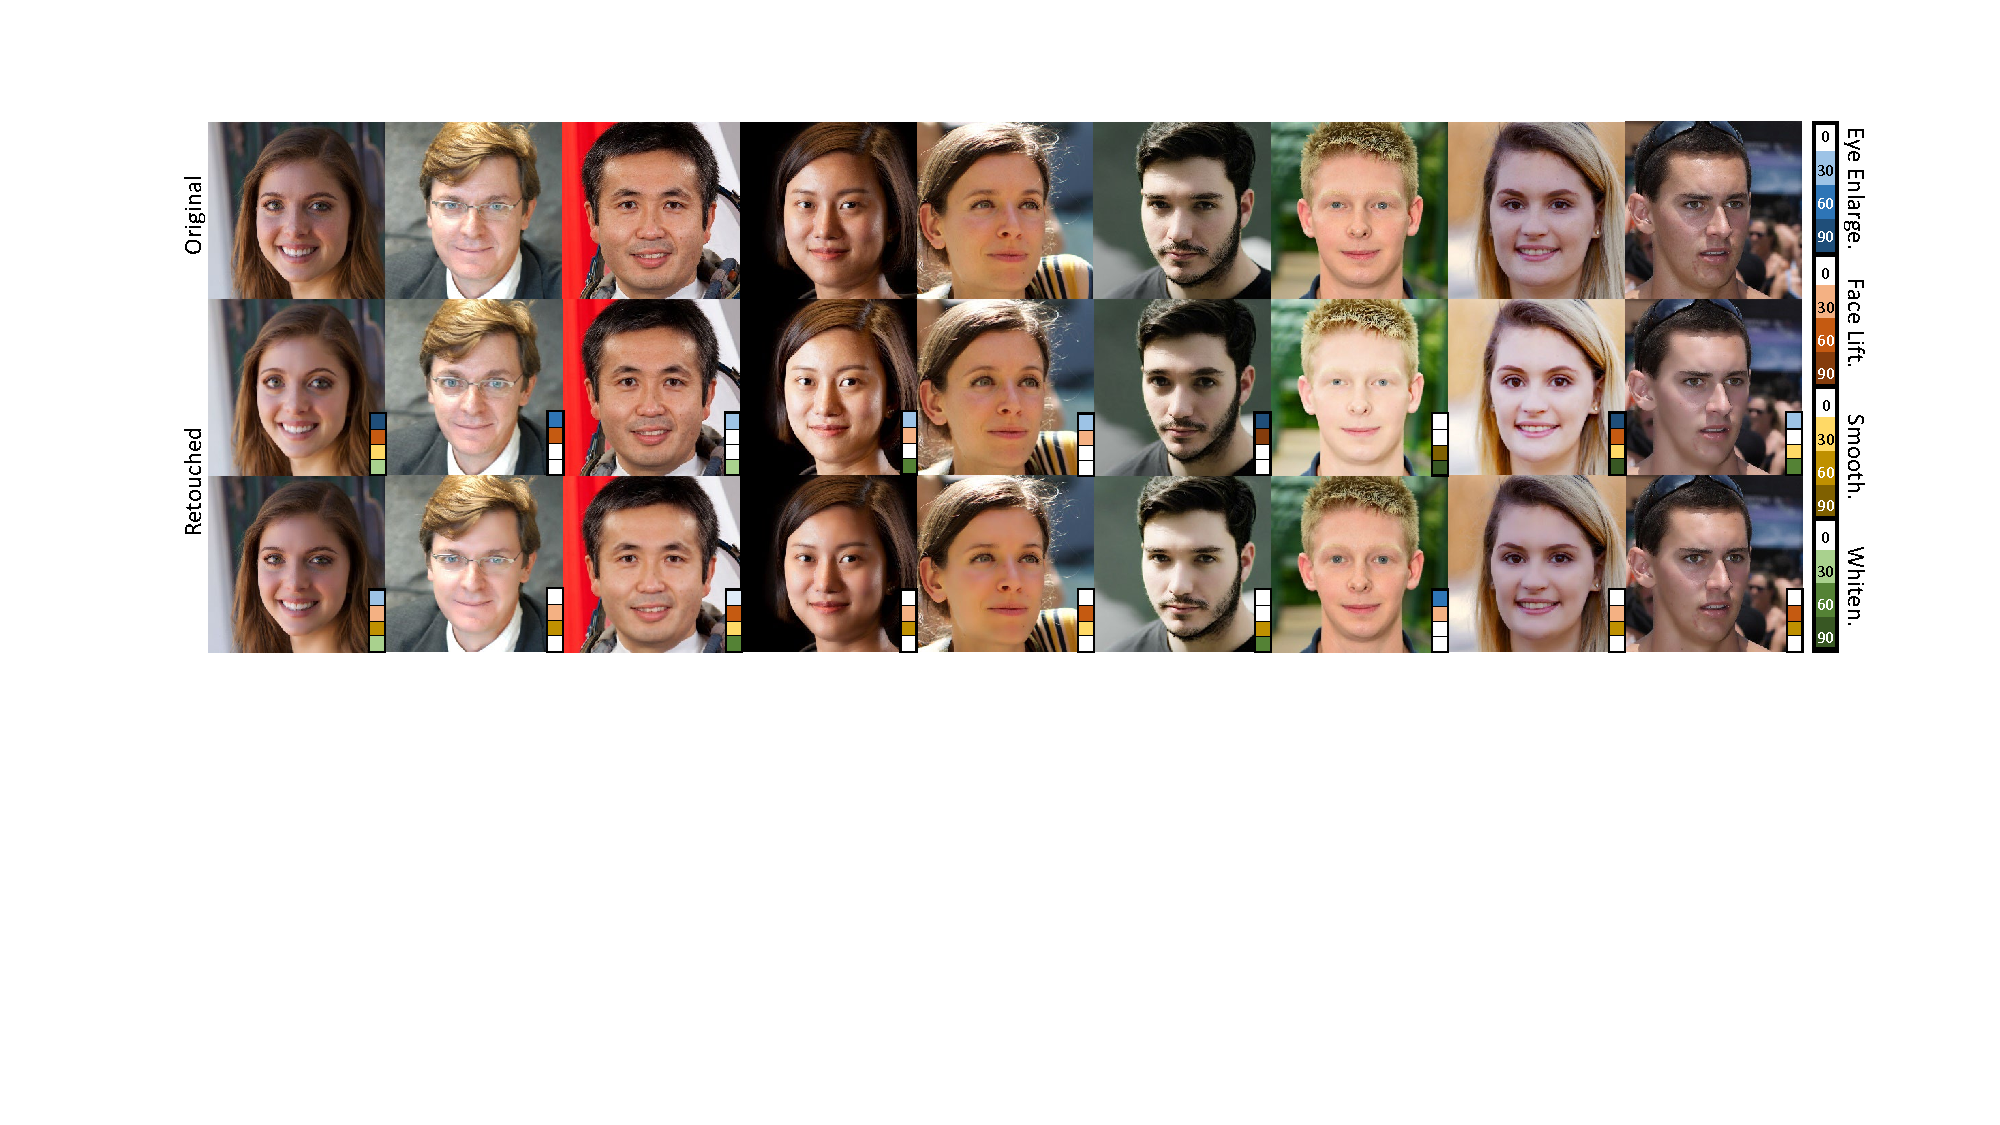
\includegraphics[width=1.0\textwidth]{figures/dataset_examples_modified.pdf}
	\caption{More examples of the dataset containing two to four operations. Labels are visualized in the downright corner.}
	\label{fig:more_example}
\end{figure*}

% \noindent\textbf{Face Manipulation Detection.}
% A number of methods have been proposed to detect face manipulations, or DeepFake. Also, there are a number of high-quality DeepFake datasets, such as WildDeepFake~\cite{zi2020wilddeepfake}, FaceForensics++~\cite{rossler2019faceforensics++} and Celeb-DF~\cite{li2020celebdf}.
% % , such as Photoshopped images~\cite{PS} or deepfake images~\cite{li2020facexray,zhao2021PCL}.
% % Wang et al.~\cite{PS} propose a dataset consisting of over 942k automatically-photoshoped images for deep networks to learn traces left by Adobe Photoshop.
% Many effective DeepFake detection networks are built on top of InceptionNet~\cite{inceptionv2}, e.g., Wang et al.~\cite{wang2020cnn}, ResNet backbone~\cite{ResNetv2}, e.g., FaceForensics++~\cite{rossler2019faceforensics++}, or EfficientNet~\cite{tan2019efficientnet}, e.g., Zhao et al.~\cite{zhao2021multi}.
% % These architectures are reported to be powerful in learning human face priors.
% % Masi et al.~\cite{masi2020two} adopt a two-stream network structure to jointly extract face representations in the frequency and spatial domain. 
% % Besides image-domain detection, there are also video-based DeepFake detection studies~\cite{liy2018exposingaicreated,mittal2020emotions,afchar2018mesonet}. 

% Face retouching detection shows exclusive characteristics with DeepFake detection and many other face manipulation detections. 
% First, face retouching detection is better to be in fine-grained form since moderate face retouching is acceptable in most scenarios. 
% In comparison, face manipulation detections are mostly in binary forms.
% Second, most decisive clues for DeepFake detection lies in the inconsistencies between fake and genuine regions~\cite{chai2020makes,zhang2022patch,li2020face,Schwarcz2021finding}.
% % For instance, Chai et al.~\cite{chai2020makes} extract the subtle manipulated traces located in the image patches. 
% % Zhang et al.~\cite{zhang2022patch} take the patch importance and correlations into consideration to learn the patch features.
% % Li et al.~\cite{li2020face} examine the face blending boundary as an additional indicator. 
% % Schwarcz et al.~\cite{Schwarcz2021finding} generate masks of the important parts of the face image to perform multi-part detection. 
% In contrast, common face retouching, e.g., smoothing and whitening, are less likely to cause artifacts and therefore rely on more higher-level feature analysis for detection.
% We build baseline models and propose a multi-granularity attention module to improve the performances.

% However, the additional challenge of detecting retouching behaviors compared to the above two tasks are mainly two-folded.
% First, typical retouching such as smoothing or whitening require less amount of modification and therefore leave less room for noticeable artifacts. 
% Second, many applications of face retouching also naturally include lossy operations, such as motion blurring or JPEG compression in livestreams.
% This could wipe out traces left by face retouching.
% Thus, either handcrafting feature extractors~\cite{rathgeb2020prnu} or training deep networks for face retouching detection both require the collection of large-scale, high-quality and diversed retouched images. 

% Though they share distinct characters, we find that many effective DeepFake detection networks are built on top of InceptionNet~\cite{inceptionv2}, e.g., Wang et al.~\cite{wang2020cnn}, ResNet backbone~\cite{ResNetv2}, e.g., FaceForensics++~\cite{rossler2019faceforensics++}, or EfficientNet~\cite{tan2019efficientnet}, e.g., Zhao et al.~\cite{zhao2021multi}.
% These architectures are reported to be powerful in learning human face priors.
% It inspires to use these popular and transferrable classical networks as baselines for RetouchingFFHQ.

\section{RetouchingFFHQ}
% \begin{figure*}[ht]
% 	\centering
% 	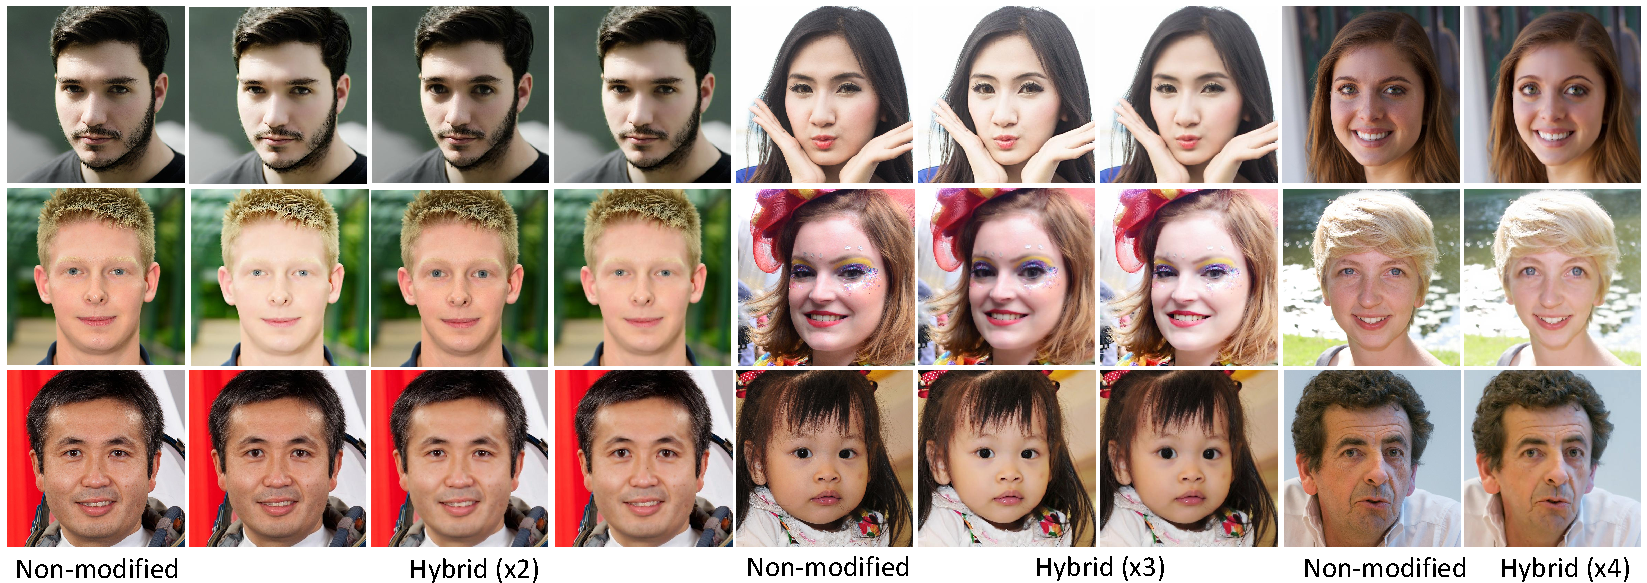
\includegraphics[width=1.0\textwidth]{figures/example_twoplus.pdf}
% 	\caption{Examples of retouched images. Better zoom in for details since for many pairs of images, the differences are trivial.}
% 	\label{fig_example_one}
% \end{figure*}
This section introduces the collection and annotation process of RetouchingFFHQ, which is based on the Flicker-Faces-HQ dataset. 
The original FFHQ dataset contains 70,000 face-aligned images sized $1024\times~1024$ collected from the Flicker dataset~\cite{FFHQ}.
Due to its large quantity of high-quality face images and variety \& balance of ages, ethnicities, genders and backgrounds, we choose FFHQ as the source to build our new dataset.

\subsection{Data Collection and Cleaning}
\noindent\textbf{The Overall Strategy.}
To create our new dataset, we generate the fine-grained retouched images using the online commercial APIs of three famous AI companies including, Megvii~\cite{Megvii}, Alibaba~\cite{Alibaba} and Tencent~\cite{Tencent}.
For the selected APIs, we find that they all support four types of commonly-used retouching including, \textit{skin smoothing, face whitening, face lifting }and \textit{eye enlarging}.
Besides, the retouching levels of the three APIs range from zero to one or a hundred.
To quantify, we categorize the levels into four classes, namely, \textit{off} (0), \textit{slight} (30), \textit{medium} (60) and \textit{heavy} (90).
With the dataset and APIs, the collection of retouched images can be done via uploading images and queries containing type and level information.
%Though collecting retouched images from TikTok, Youtube Short or mobile Apps can be also promising, it is harder to find similar APIs for automatic and large-scale data collection.
% Second, though other operations such as \textit{acne or blemish removal} or \textit{lipstick enhancement}, we empirically find that they are usually crafted for typical types of defective images or can also be carried out by the included types, e.g., smoothing.

%%%%%% move to supplementary material
% \begin{table}[!t]
% % \renewcommand\arraystretch{1.15}
% \begin{center}
%    \caption{Dataset details and mapping rule from FFHQ to RetouchingFFHQ. $^1$: we downsample the original images to prevent overfitting on the ``non-processed" (0) class.}
%    \label{table:dataset}
% \begin{tabular}{c|c|c|c}
% 		\hline
% 		& Source Images (\#Shots) & \#\textbf{Types} & \#Excl. \\
%         \midrule
%         Single & \makecell[c]{Train:00000-16999 (68000)\\Val:00000-16999 (68000)\\Test:17000-19999 (12000)} & \makecell[c]{\textbf{4} (S, W,\\L, E)} & \makecell[c]{475}\\
%         \midrule
%         Dual & \makecell[c]{Train:20000-36999 (102000)\\Val:00000-16999 (68000)\\Test:37000-39999 (18000)} & \makecell[c]{\textbf{6} (L\_E,..., \\L\_S)} & \makecell[c]{364}\\
%         \midrule
%         Triple & \makecell[c]{Train:40000-56999 (68000)\\Val:00000-16999 (68000)\\Test:57000-59999 (12000)} & \makecell[c]{\textbf{4} (W\_L\_S, \\...,W\_S\_E)} & \makecell[c]{433}\\
%         \midrule
%         Quad & \makecell[c]{Train:60000-69999 (8500)\\Val:00000-16999 (68000)\\Test:67000-69999 (1500)} & \makecell[c]{\textbf{1} (L\_E\_ \\W\_S)} & \makecell[c]{532}\\
%         \midrule
%         Ori. & \makecell[c]{Train: Ori imgs of above (8500$^1$)\\Val: Ori imgs of above (68000)\\Test: Ori imgs of above (43500)} & / & \makecell[c]{11278}\\
% 		\hline
% 	\end{tabular}
%  \end{center}
% \end{table}

% Table~\ref{table:dataset} summarizes the dataset details and the mapping rule of images from FFHQ to RetouchingFFHQ.

\noindent\textbf{Face Image Cleaning.}
% Noisy data generally do more harm than good to the training of neural networks~\cite{noisy2019,noise_survey}.
We find that a noticeable portion of images from FFHQ are either not proper to perform retouching, or occasionally appear in real-world face retouching scenarios. These images can be mostly summarized into the following five types.% The potentially affected retouching are in the brackets.
1) Blurriness or Poor/Abnormal Lightning Condition, 
% since missing details would prevent algorithms to identify the five senses for face retouching.
2) Cosplay, Already Filtered or with Heavy Makeups, 
% since these images largely do not require further digital retouching and therefore potentially causing misclassifications. 
% Considering that many characters can carry slight makeups that escape cleaning, we only exclude those images that apparently prevent digital retouching.
3) Incomplete Faces,
% since failure of localizing the five senses would affect the retouching. Typical type are \textit{Closed Eyes}, \textit{Side Profile}, \textit{Wearing Mask/ Sunglasses/ Helmet, etc}.
% So we exclude side-profiled images and those with closing-eye temptation.
4) Images of Infants and Babies, and
% since they take a non-negligible portion, and face retouching on infants can be considered very rare and trivial.
% We find that the face outlying of infants and tutors are characterized by circle-shape and smooth skin, which largely deviates from those of adults. As a results, their retouched images are mostly weird-looking. Besides, it is less likely for them to use beautifying filters.
% 5) \textit{face Coverage} (affecting all operations),
% because of wearing mask, sunglasses, helmet, etc. 
% As a result, some of the beautifying operations might not work.
    % \item \textbf{Multiple Actors (All Operations).} We find that when there are multiple actors, it is uncertain that which face will be modified by the beautifying algorithms. Therefore, to mitigate under-training, we remove these images. 
5) Fake Faces.
% where some face images are captured from magazines, sculptures or cartoon characters.
% Bearing these rules for spotting OOD samples in mind, 
We manually check all the 70k images in FFHQ and remove the face images which belong to the five categorizes mentioned above. After the cleaning, we construct an original face image dataset with 58158 samples captured from 58158 different persons. 
% We store the indices of the excluded images in separate text files according to the above categories. 
%\needattention{Their indices and representative examples are shown in the supplementary material}.
% Please note that by data cleaning, we also acknowledge that the trained models would predict unconvincing results if encountered with the above-listed ood examples.  

% \begin{figure}[!t]
% 	\centering
% 	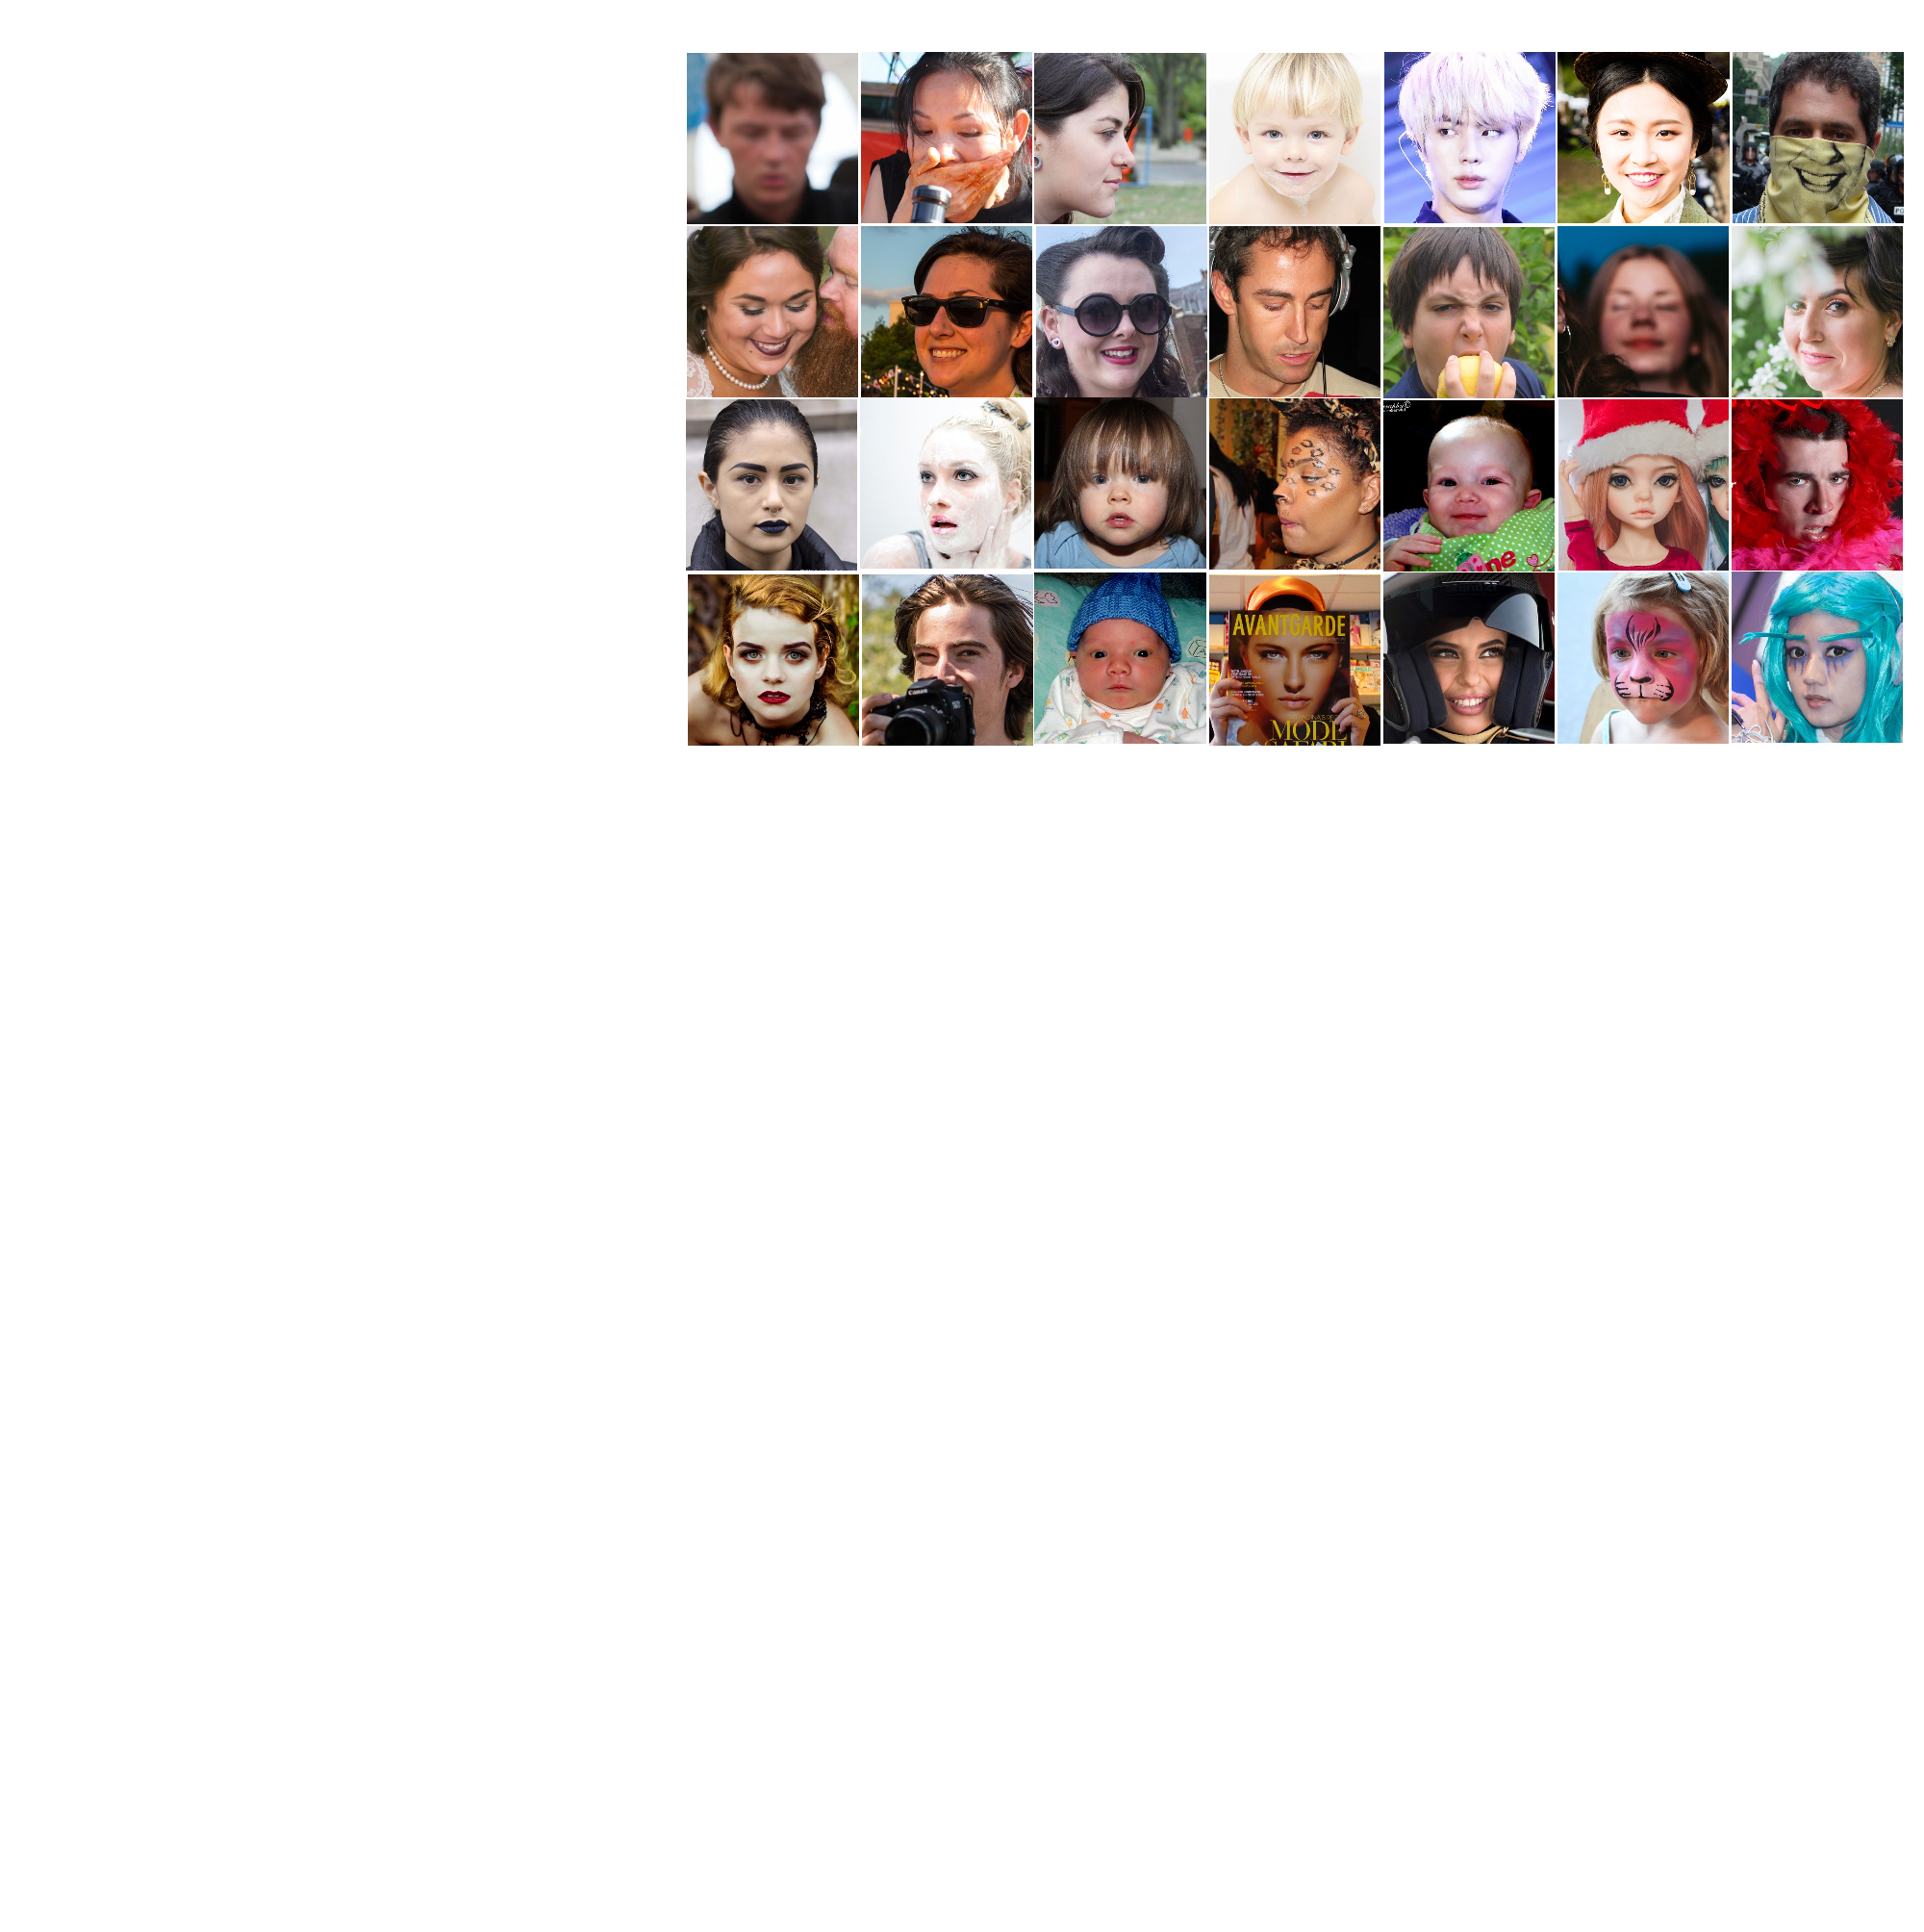
\includegraphics[width=0.48\textwidth]{figures/ood.pdf}
% 	\caption{Examples of ruled-out original images, which are mostly over-exposed, with sunglasses or heavy make-ups that prevents successful digital face retouching.}
% 	\label{fig:ood}
% \end{figure}

\noindent\textbf{Retouched Face Image Collection.}
We split the cleaned original images into four non-overlapping subsets according to their indices in FFHQ, where images indexed 0-20k belong to the first subset, 20k-40k to the second, 40k-60k to the third, and 60k-70k to the last. 
% % (\texttt{00000}-\texttt{69999}), 
% % and split them into non-overlapping four parts with respectively 20k
% % (\texttt{00000}-\texttt{19999})
% , 20k 
% % (\texttt{20000}-\texttt{39999})
% , 20k 
% % (\texttt{40000}-\texttt{59999}) 
% and 10k 
% % (\texttt{60000}-\texttt{69999}) 
% images. 
% Then, the first part is allocated for the generation of single-operated images, i.e., images which only contain one type of retouching, and the second part for dual-operated images, the third part for triple-operated images, and the fourth part for quad-operated images.
We perform different amount of retouching operations for different original image subsets, the details of which are given below.
\begin{itemize}
\item \textbf{Subset-0} (\textit{Non-retouched images}): The subset is composed of the above cleaned images without any digital retouching.
\item \textbf{Subset-1} (\textit{Single-operated images}): Each original face image is individually retouched into four retouched versions by respectively applying one type of retouching, and the levels are evenly drawn from off (0), slight (30), medium (60) and heavy (90). Exampled images are \textit{skin-smoothed} images, \textit{eye-enlarged} images, etc. 
\item \textbf{Subset-2} (\textit{Dual-operated images}): Each original face image is individually retouched into six ($C_4^2$) retouched versions by respectively applying two type of retouching.
The levels of each performed retouching are also evenly and independently drawn from the three positive classes. Exampled images are \textit{skin-smoothed \& face-lifted} images, \textit{eye-enlarged \& face-whitened} images, etc. 
\item \textbf{Subset-3} (\textit{Triple-operated images}): Each original face image is individually retouched into four ($C_4^3$) retouched versions by respectively applying three type of retouching.
The levels are also evenly and independently drawn. Exampled images are \textit{skin-smoothed \& face-lifted \& eye-enlarged} images, etc. 
\item \textbf{Subset-4} (\textit{Quad-operated images}): Each original face image is retouched by applying all four retouching operations and the levels are evenly and independently drawn.
Because there are less original images in this subset, we generated two different retouched versions for each sample.
\end{itemize}

% It is well notifying that there exist circumstance where for an image, the effects of different levels for a certain retouching, e.g., 30 and 60 for smoothing, are close. 
\begin{figure*}[!t]
	\centering
	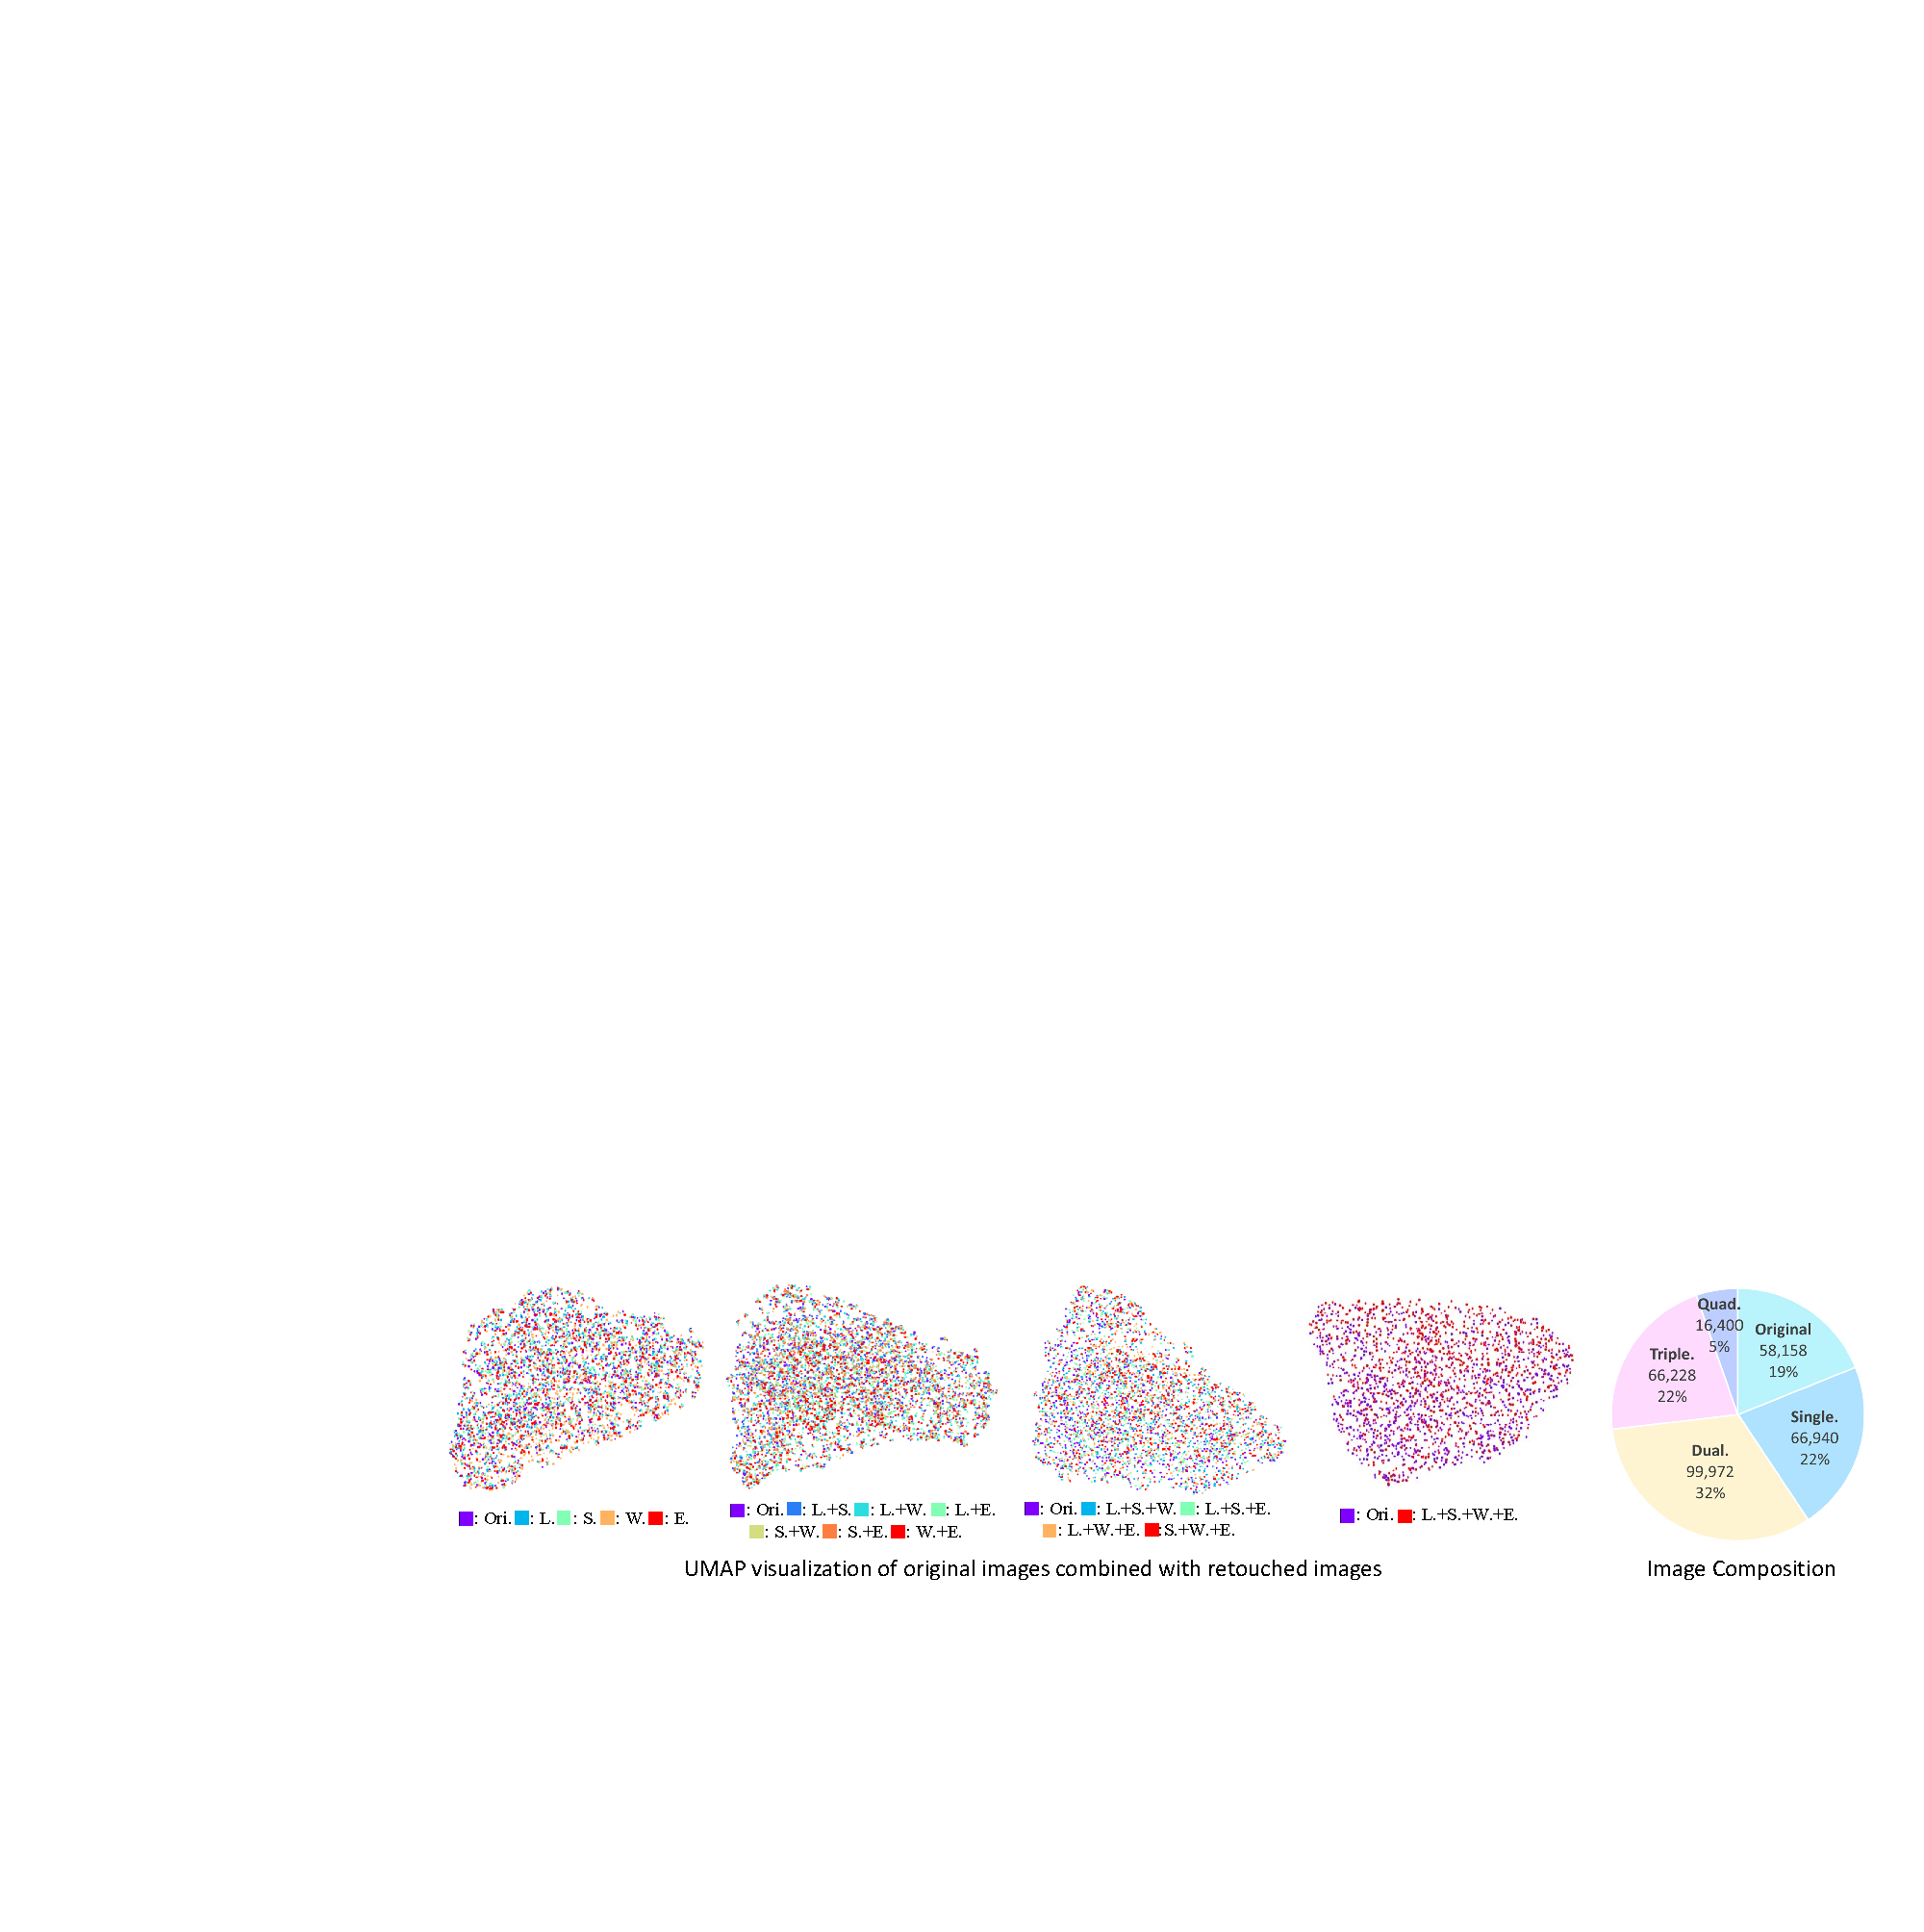
\includegraphics[width=1.0\textwidth]{figures/data_statistic.pdf}
	\caption{UMAP visualization and image composition of the Megvii retouching subset.}
	\label{fig:umap}
\end{figure*}
\begin{figure}[!t]
	\centering
	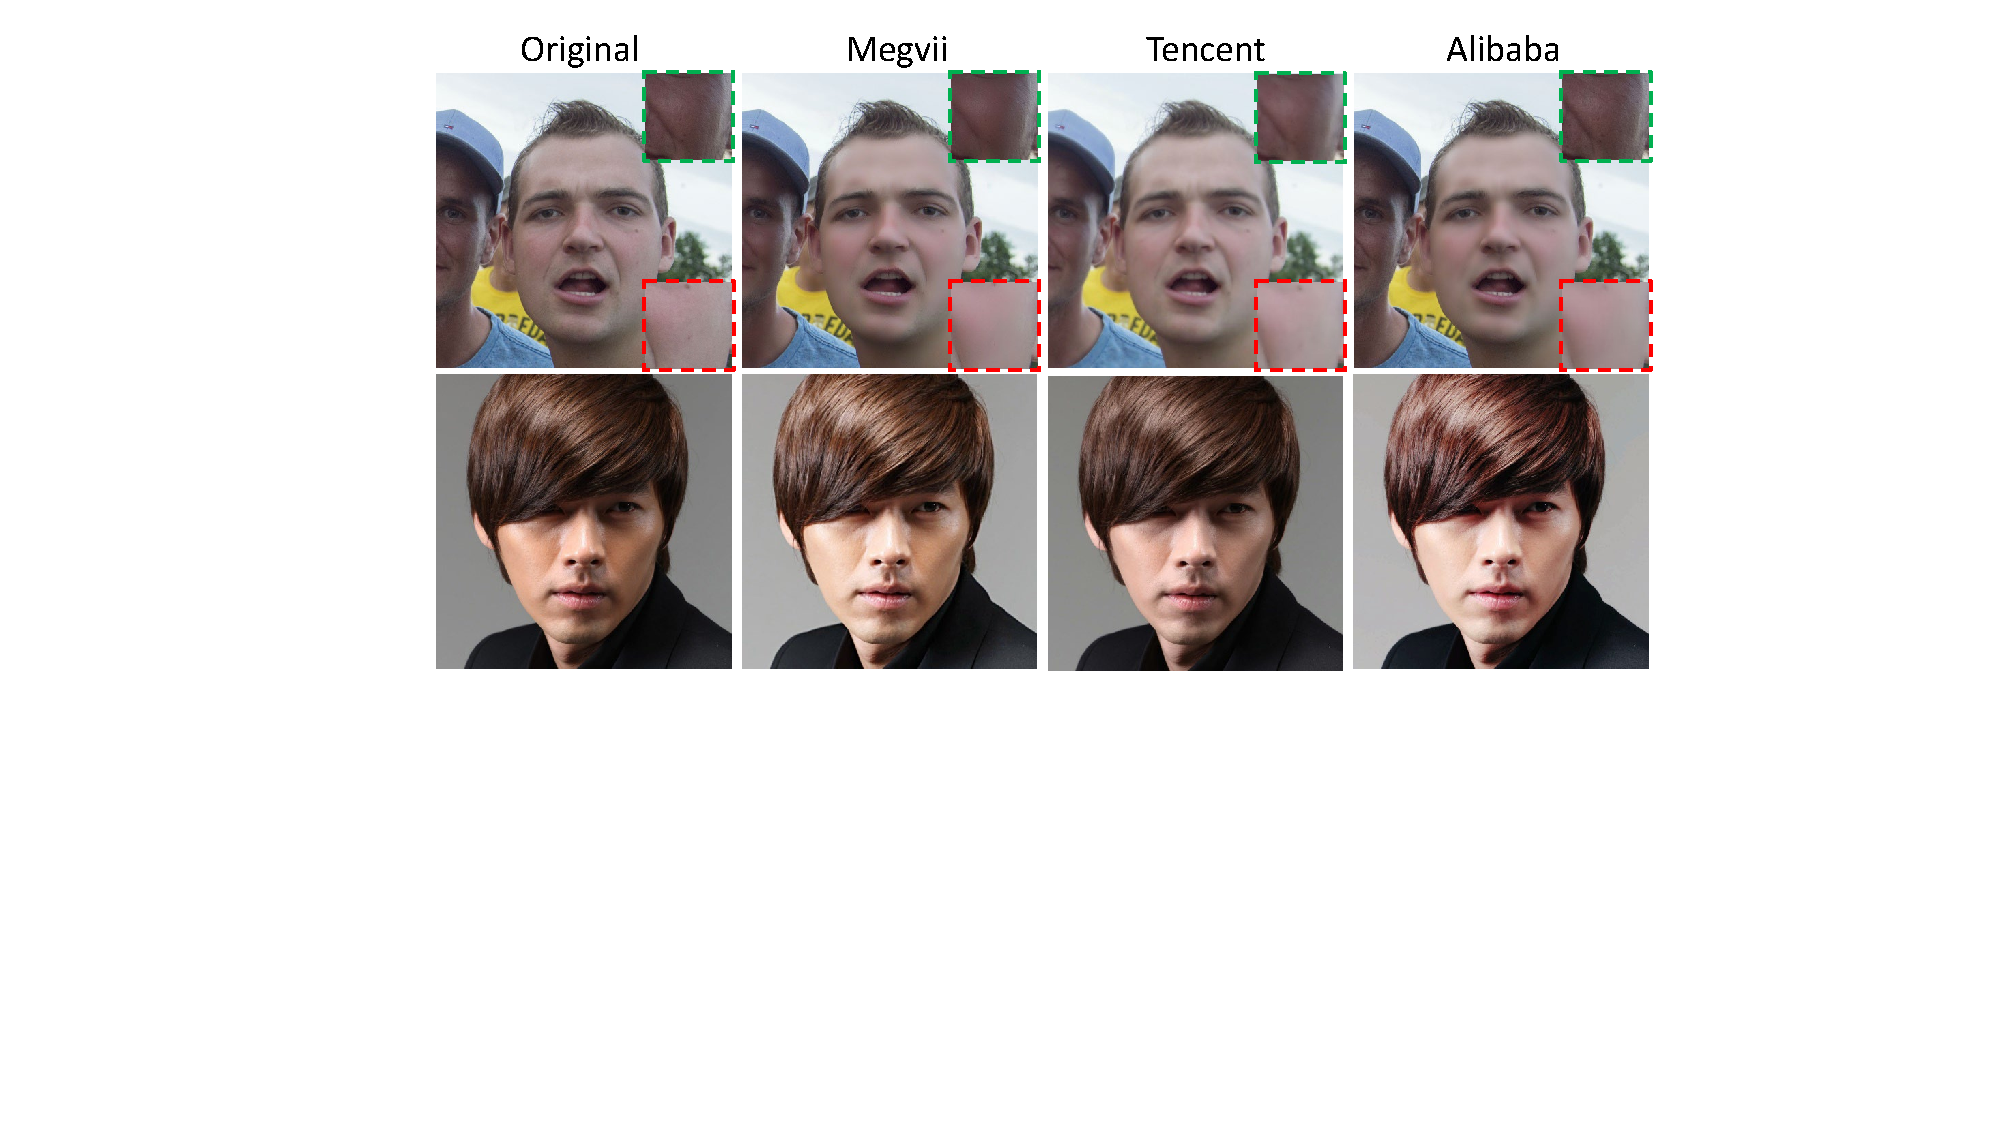
\includegraphics[width=0.48\textwidth]{figures/API_diff.pdf}
	\caption{Examples of differences in visual effects among APIs. Annotations: (Upper) Smooth 90. (Lower) Smooth 90. Please zoom in to see differences in details and color.}
	\label{fig:API_diff}
\end{figure}
Besides the division according to the amount of retouching, RetouchingFFHQ can also be divided into three sets according to the source API of the images, namely, the \textbf{Megvii set}, the \textbf{Tencent set}, and the \textbf{Alibaba set}.
We save all the collected images in a uniform resolution $512\times~512$.
Notice that the Alibaba API only allow performing one retouching at a time, and thus we only collect the single-operated images in this subset.
Also, for Subset-1 of the Alibaba and Tencent set, we additionally provide images of each type in all three levels, resulting in two times more single-operated images.
Table~\ref{tab:dataset_summary} summarizes RetouchingFFHQ, which counts all subsets of the images reports the average PSNR between original images and their retouched versions w.r.t different APIs and the amounts of operations. Fig.~\ref{fig:more_example} showcase more examples of retouched faces randomly drawn from Subset 2-4, where the labels are attached in the downright.
% We provide more examples in Fig.~\ref{fig:more_example}, where the source APIs are harder to discern.
% Nevertheless, the discrepancies can potentially pose challenges in the generalizability of unified face retouching detection. 

\noindent\textbf{Data Splitting.}
We split the original face images (and their corresponding retouched versions) in our RetouchingFFHQ into training, validation and testing sets with a ratio of 80\%, 10\%, and 10\%. 
% In sum, the whole dataset contains 35k, 5k, and 5k images in each group, respectively.
% For the original images, we prevent the leakage of prior information by 

% \needattention{The discrepancies between different APIs are showcased in the supplementary material.}

% While individual APIs contain filters or other operations such as eyebrow lifting or cheekbone lifting, they are generally unique.
\subsection{Annotation and Objective Function}
% Each face image is annotated by the following form: {\texttt{Smooth}: $s$,\texttt{EyeEnlarge}: $x$,\texttt{FaceLift}: $y$,\texttt{Whiten}: $z$\}, where $w$, $x$, $y$ or $z$ refer to the retouching level of each single operation with 0 being not retouched, 1 being slight retouched, 2 being medium retouched, and 3 being heavy retouched. For example, if a face image is retouched using medium eye-enlarging and heavy whitening. Its annotation would be \{\texttt{Smooth}: 0, \texttt{EyeEnlarge}: 2, \texttt{FaceLift}: 0, \texttt{Whiten}: 3\}. \li{(...tell people what is slight, medium and heavy in the previous section...)}
\noindent\textbf{Annotation.} Each face image is annotated in the following form: 
\begin{equation}
    \{\texttt{Smooth}: s,\texttt{EyeEnlarge}: e,\texttt{FaceLift}: l,\texttt{Whiten}: 
    w\},
    \nonumber
\end{equation}
where $s$, $e$, $l$ or $w$ refer to the retouching level of each single operation.
We use zero to denote the ``off (0)" class, one to denote the ``slight (30)" class, two to denote the ``medium (60)" class, and three to denote the `` heavy (90)" class.
For instance, if a face image is retouched using medium eye-enlarging and heavy whitening. Its annotation would be therefore $
    \{\texttt{Smooth}: 0,\texttt{EyeEnlarge}: 2,\texttt{FaceLift}: 0,\texttt{Whiten}: 
    3\}$.
% It is better than multi-class classification with a single label, as it allows for the use of independent classifier to detect different types of retouching.

% \noindent\textbf{Multi-label Objective Function.}
\noindent\textbf{Objective Function.}
For detection networks, we adopt an emsemble of four separate Multi-Layer Perceptrons (MLPs), where each MLP predicts the retouching level of a certain type. These MLPs are trained together in a multi-task manner. The overall loss function is an aggregation of four Cross-Entropy (CE) losses designed for the four MLPs, which is formulated in Eq.~(\ref{eqn:CE}).
% \begin{equation}
% \label{eqn_jpeg}
% \mathcal{L}_{\emph{sum}}=\sum_{l=1}^{4}\emph{CE}(\mathbf{P}_{o},\mathbf{P}_{r})=-\sum_{l=0}^{3}\sum_{\emph{level}=0}^{3}y_{o,c}\log(p_{o,c}),
% \end{equation}
% where $y$ is the binary indicator if class label $c$ is the correct classification for observation $o$. $p$ is the predicted probability observation $o$ is of class $c$. $\mathbf{P}_{o}$ takes the \textit{argmax} of $o$ that maximizes $p$.
\begin{equation}
\label{eqn:CE}
\mathcal{L}_{\emph{sum}}=\sum_{t\in\{S,E,L,W\}}\emph{CE}(\mathbf{Y}_{t},\mathbf{P}_{t})=-\sum_{t} \sum_{\emph{l}=0}^{3}y_{t,l}\log({p}_{t,l}),
\end{equation}
where $p_{t,l}$ is the predicted probability for type $t$ and level $l$, and $y_{t,l}$ is the ground-truth level. 
% $\mathbf{\hat{P}}_{t}$ takes the \textit{argmax} of $t$ that maximizes $p$.


\subsection{Statistics and Visualizations}
% In Table~\ref{tab:dataset_compare}, we further show the average PSNR between original images and their retouched versions w.r.t different APIs and the amounts of operations.
% We see that though more operations lead to lower averaged PSNR, the gaps are not remarkable as expected.
% RetouchingFFHQ includes over half a million retouched images which can be categorized into different groups according to either the amount of operated retouching or the source API.
\noindent\textbf{API Discrepancies.}
First, we find that the three APIs differ in the visual effects, as showcased in Fig.~\ref{fig:API_diff}.
It is mainly due to the characteristics of the underlying algorithms, as well as how levels correspond to the extent of modifications.
Therefore, besides mixing all retouched images from the three APIs as a whole to train joint models, we can also train them on the basis of a single API and conduct cross-API verification to test the generalization.
% the Tencent API tends to apply smoothing and whitening globally, while the Megvii API mainly perform the operations within the face areas.
% Users can either use all subsets of the retouched images to train unified models for detecting images with different amounts of operations,
% or use a portion of them for specific applications, e.g., using Subset-4 for the detection of highly retouched images.

\noindent\textbf{Visualizations.}
We demonstrate the inter-category variability in Fig.~\ref{fig:umap} by randomly selecting 1000 original images and the corresponding retouching images from the Megvii dataset. 
We use a pretrained FaceNet model~\cite{facenet} to extract face representations and UMAP~\cite{UMAP} for visualization.
We see that the reduced features are mainly clustered with little inter-class discrepancies, suggesting that the retouching usually introduces moderate modification that poses challenges to face retouching detection. 
% Also, the image composition of the Megvii set is shown, which is with a comparatively balanced data ratio similar to the real-world situation.
% Each portion contains at least 16k retouched images.

% \noindent\textbf{Discussions.} 
% Although we filtered out OOD examples, e.g., those with apparant makeups, it is challenging for the complete removal of noisy data, i.e., there must exist images with slight makeups that escaped data cleaning.
% OOD detection could be a promising direction~\cite{VOS,liu2020energy}.
% However, this category lack enough data for balanced training.
% We leave it future works.

% \noindent\textbf{Ethical Consideration.}
% All retouched images within RetouchingFFHQ are granted by the three involved companies and intended for research purposes only.
% The images as well as data processing scripts will be made available after the undergoing anonymous reviewing process. By data cleaning, all volunteers have agreed that they will not be influenced by ethical concerns such as gender, nationality, race, etc.

% \begin{figure*}[ht]
% 	\centering
% 	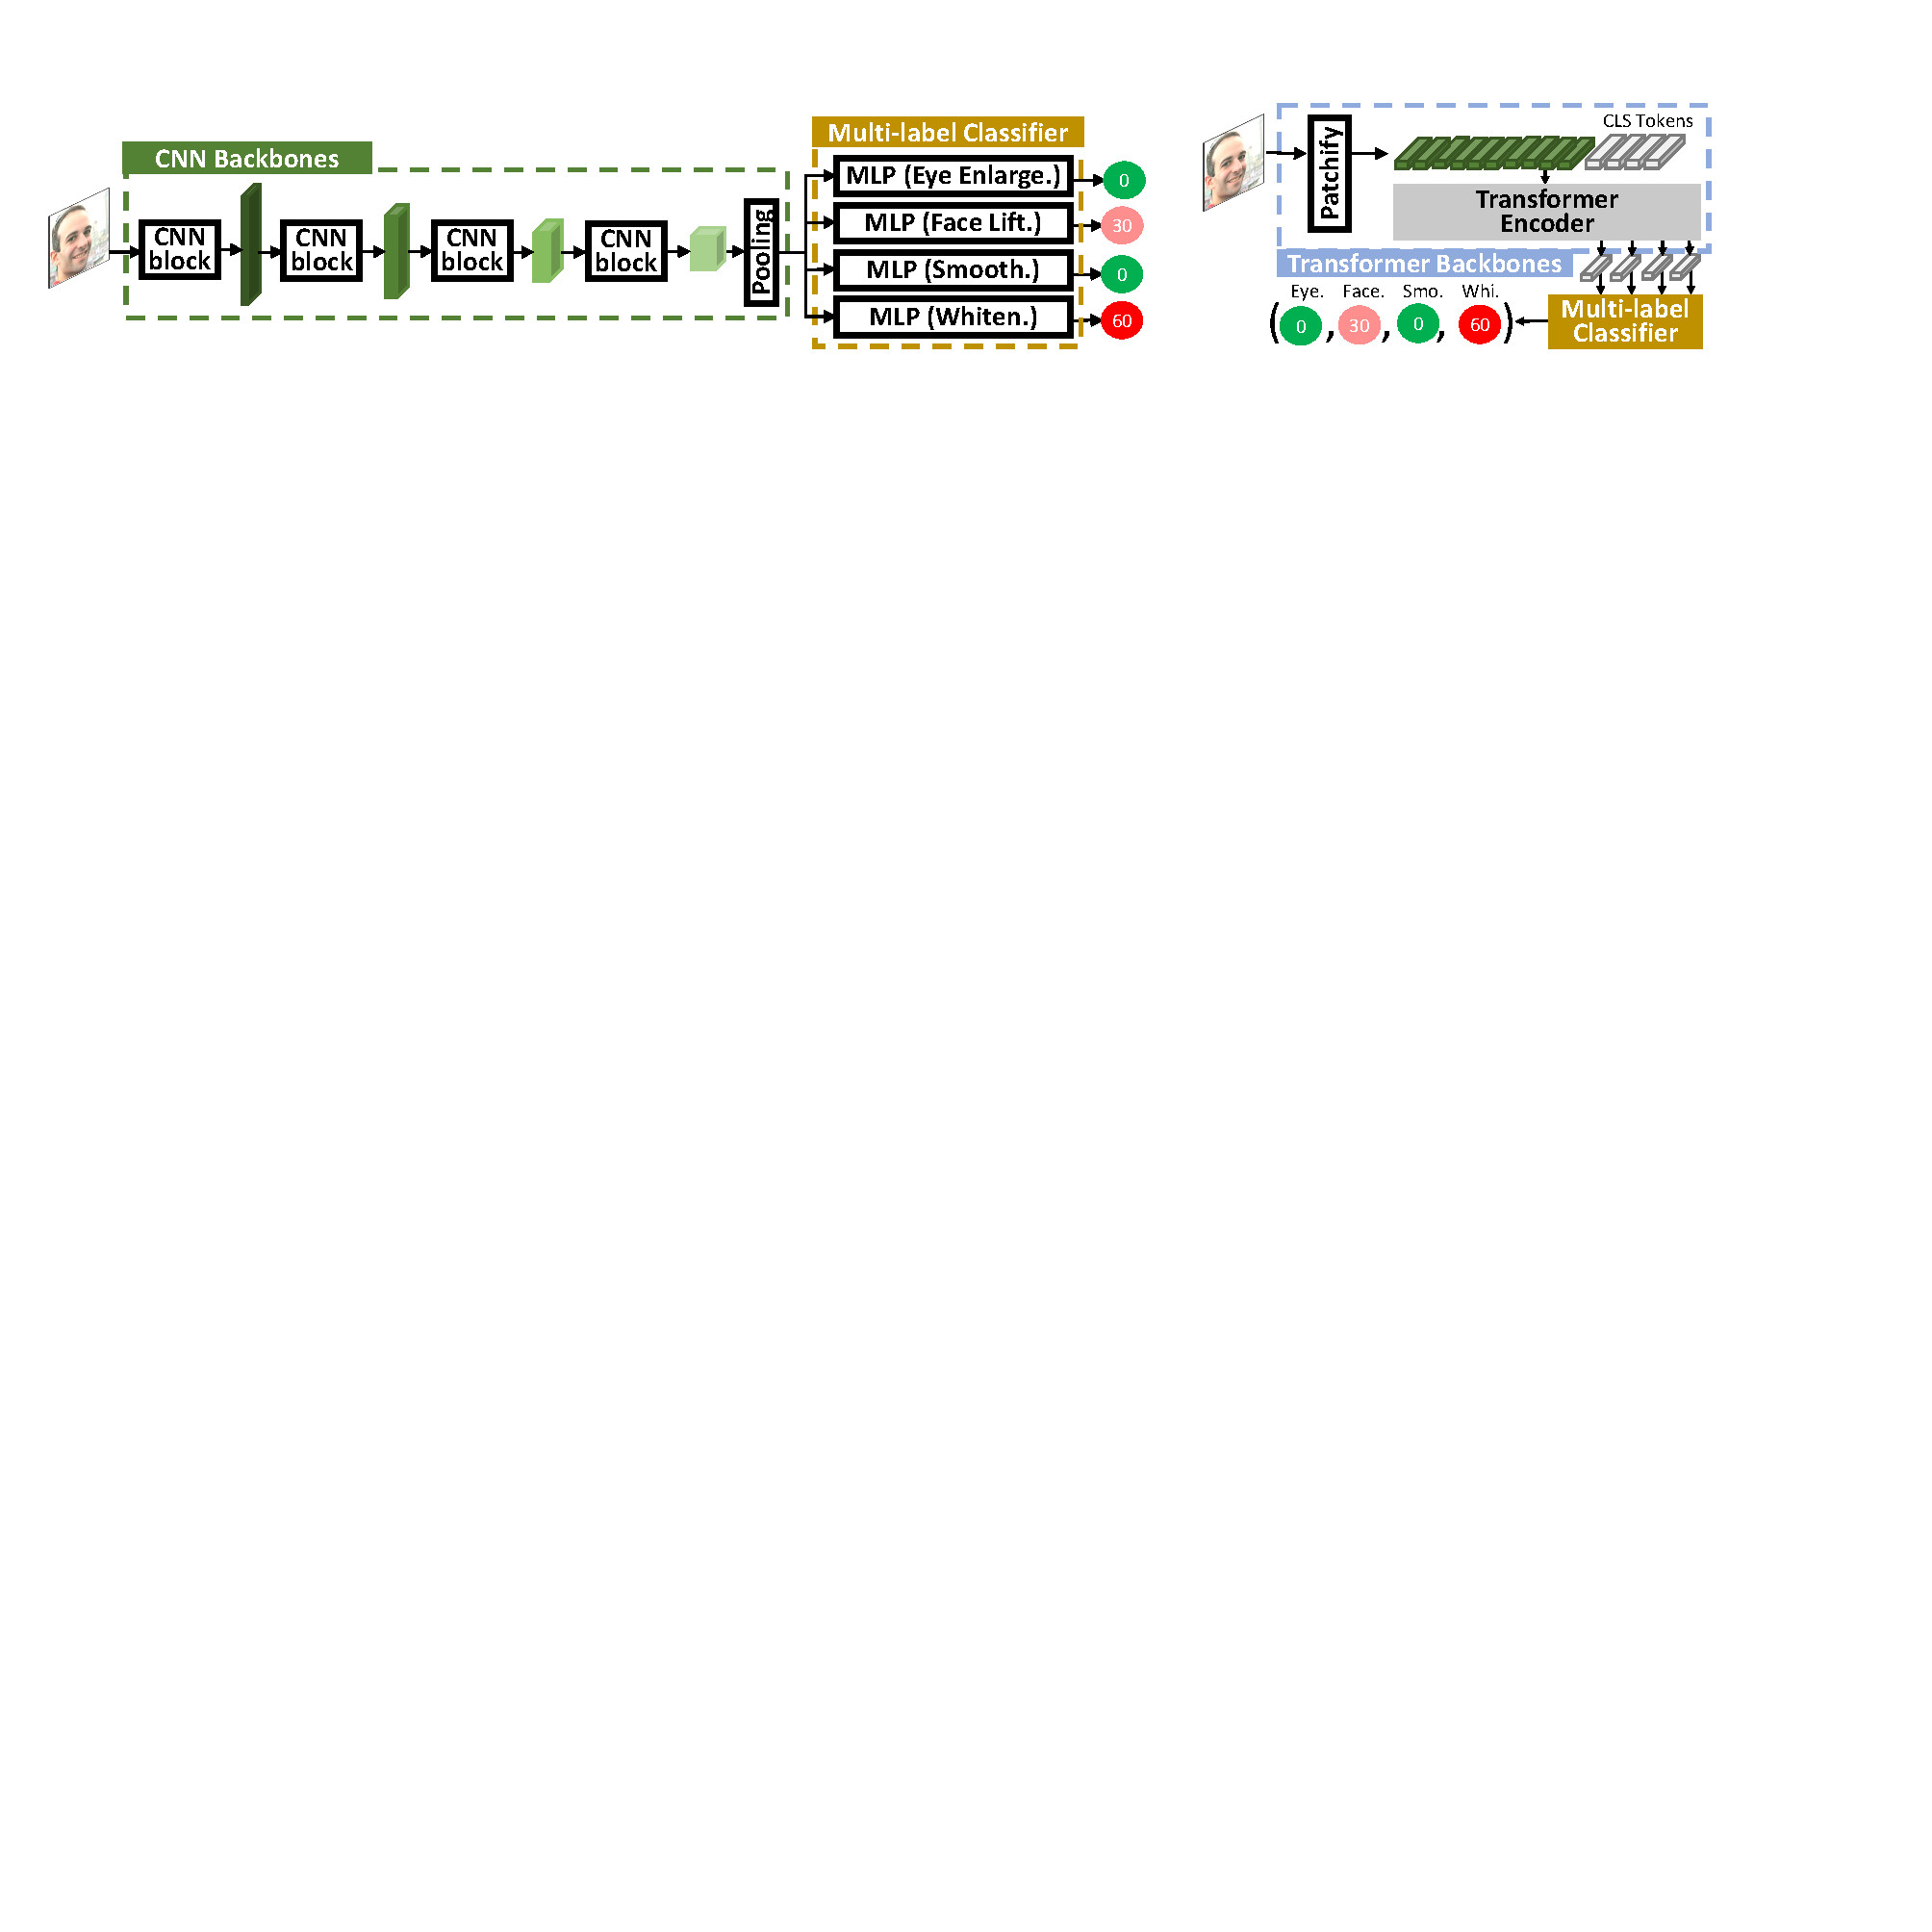
\includegraphics[width=1.0\textwidth]{figures/baseline.pdf}
% 	\caption{Baseline architectures both with multi-label classifiers. Left: using CNN backbones. Right: using Transformer backbones.}
% 	\label{fig:network}
% \end{figure*}
% \begin{figure}[!t]
% 	\centering
% 	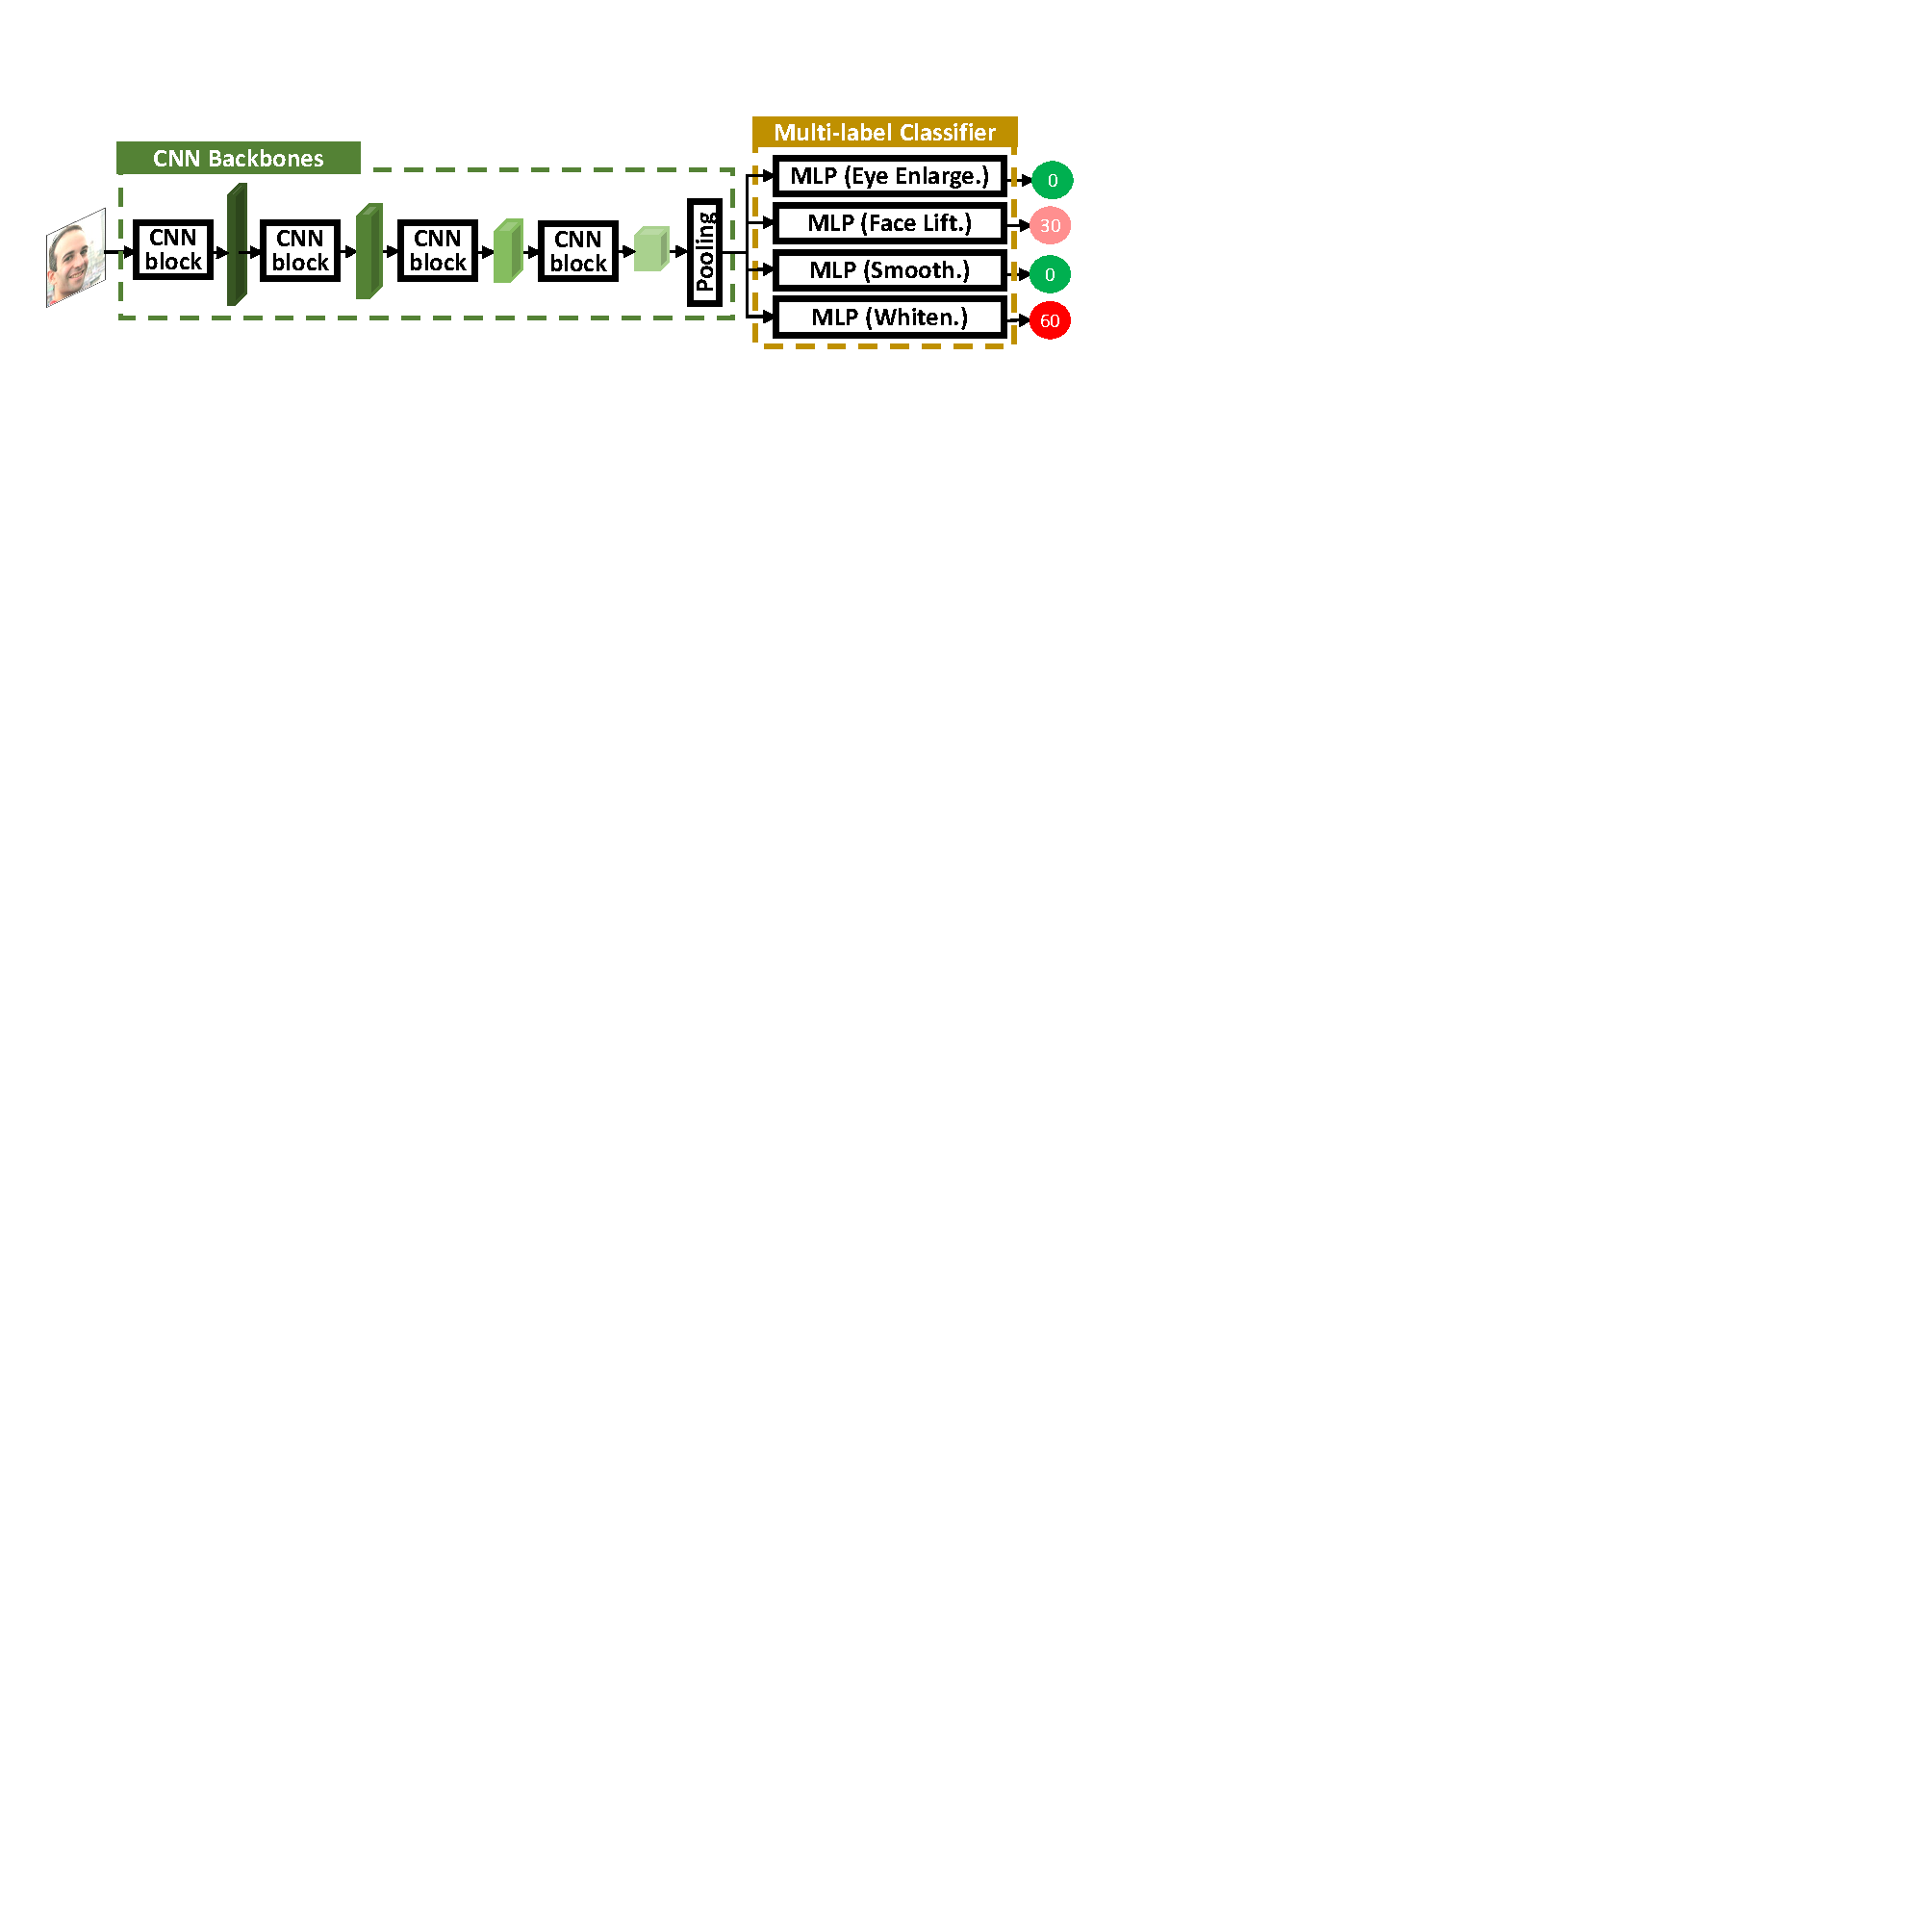
\includegraphics[width=0.5\textwidth]{figures/network.pdf}
% 	\caption{CNN baselines with multi-label classifier.}
% 	\label{fig:intuition}
% \end{figure}

\section{The Multi-granularity Attention}
\label{section:MAM}
% \noindent\textbf{Problem Statement.}
% We propose MAM as a plug-in to improve the performance of deep network in face retouching detection.
% \subsection{Problem Statement}
\noindent\textbf{Multi-granularity in Face Retouching Detection.}
We investigate how humans make predictions without reference to the original faces by scrutinizing the retouched images as shown in Fig.~\ref{fig:more_example}.
Besides geometric distortion or noise-level artifacts left by retouching algorithms,
% In this point, CNNs are already proven excellent in pattern recognition, but the advancement of generative networks can be promising in alleviating such defects.
% geometric distortion and noise-level artifacts can also be erasable by lossy image compression.
we find that the other critical factor relies on the features that can be learnt from multiple granularities. For instance, given an image with large eyes shown in Fig.~\ref{fig:more_example} (row 1, column 1), a closer look on the eyes would easily lead to the conclusion that the image has undergone eye-enlarging. 
However, further considering the large occupation of the face in the image as well as the reasonable ratio of eyes and face, we would reconsider the image as not being eye-enlarged.
%Also, closer look on the skin of image in row 3, column 9, would tell that there are little details, but it could also because of image compression.
%Further, we find that the patches representing the T-shirt contain fine details, and we are thus more convinced that the image has undergone face smoothing.
Similar phenomenon could also be observed on other retouching types.
Besides, there can exist a non-negligible amount of spatial redundancy within the visual representations. For example, the background and skin regions can be reduced into two tokenized representation containing the averaged statistic of lightning condition and sharpness.

\begin{figure}[!t]
	\centering	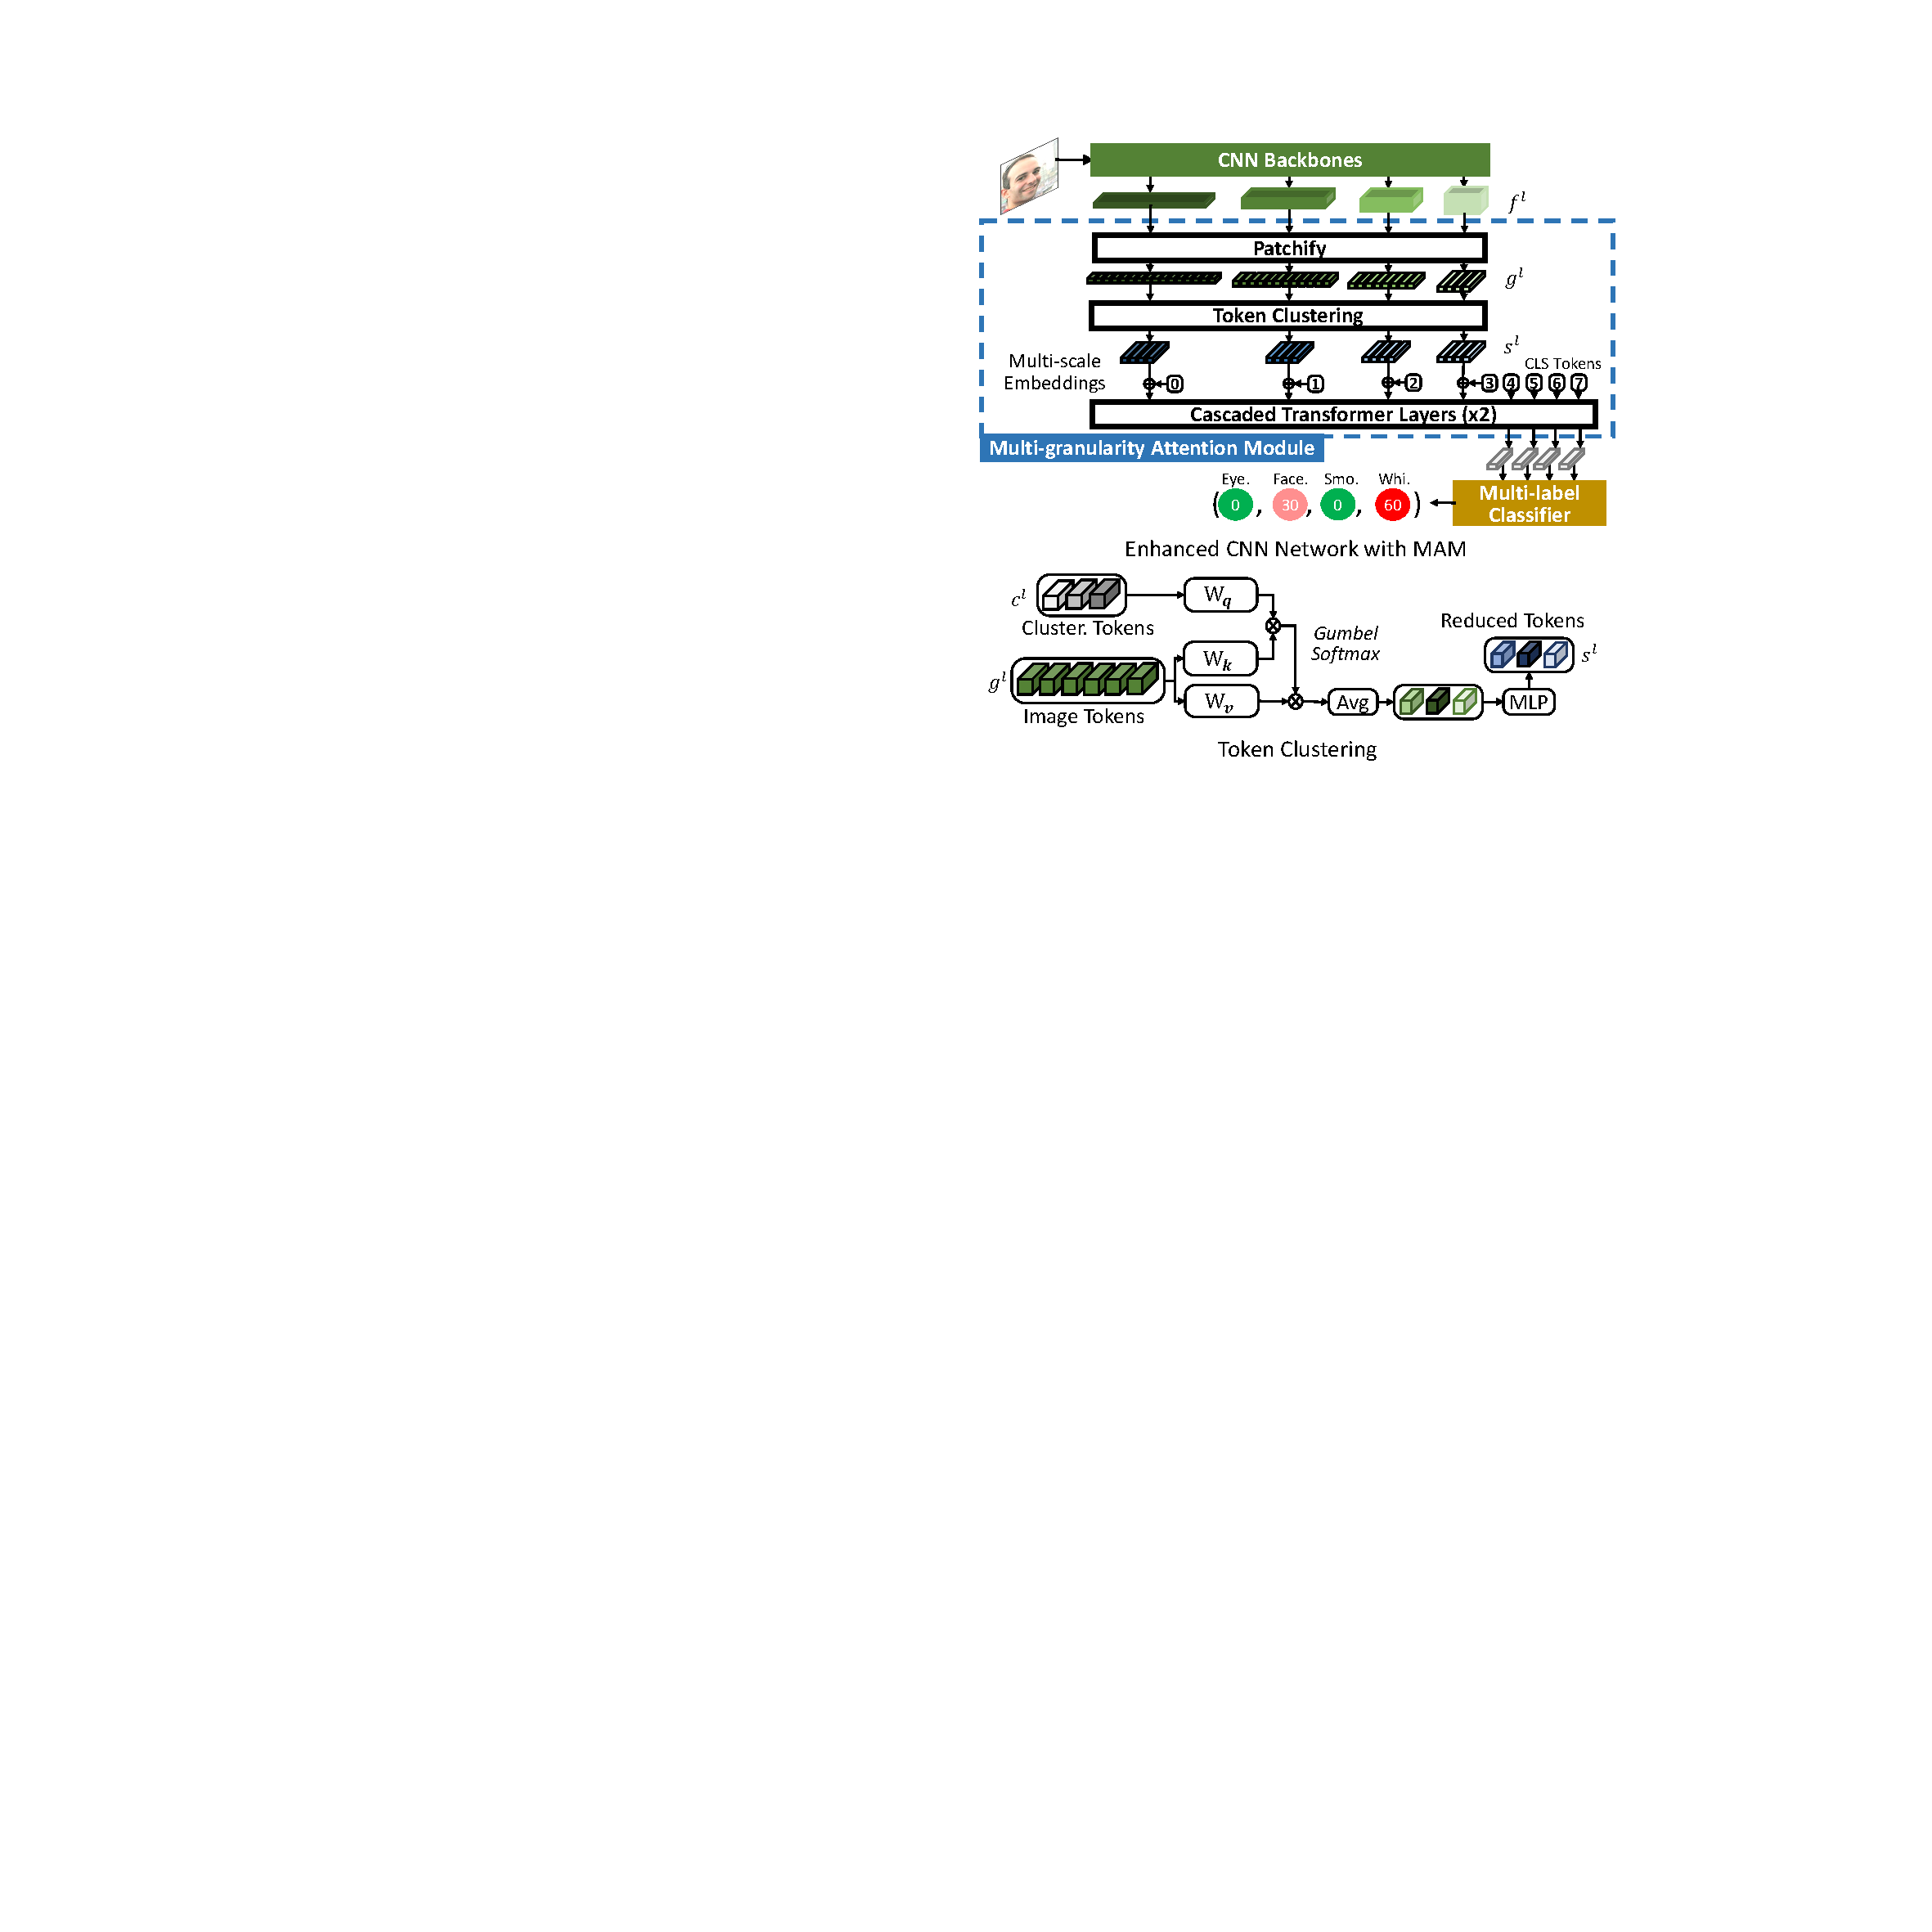
\includegraphics[width=0.48\textwidth]{figures/intuition_new.pdf}
	\caption{Network Design of the proposed MAM.}
	\label{fig:intuition}
\end{figure}
As shown in Fig.~\ref{fig:intuition}, for spatial redundancy reduction, we propose the adaptive token clustering method.
For enhanced multi-granularity representation learning, we employ a lightweight two-layered Transformer encoder~\cite{Vaswani2017attention} to analyze and compare multi-granularity information for detection. 
% \li{why do we need to reduce the redundency?} 
% Next, we elaborate the methodology in detail. 

% In the below, we present two designs of MAM as plugins to CNN networks.
% \subsection{Multi-granularity Attention Module}
% The design of MAM consists of two cascaded stages, namely, redundancy reduction and co-attention.

% \noindent\textbf{Feature Calibration.}
% Because the hierarchical features simultaneously deliver information for the whole backbone and MAM, we follow the principle of \cite{self_distill,other} to calibrate each level of the multi-scale features using one separate residual block~\cite{residual}.
\noindent\textbf{Adaptive Token Clustering.}
%\noindent\textbf{Redundancy Reduction via Token Clustering.}
% This inspires us that the representations can be reduced in size before performing cross-scale co-attention.
% We propose two ways for such redundancy reduction.
% \noindent\textbf{Adaptive Reduction: Token Clustering and Projection.}
% The TMAM takes the token-clustering-based adaptive reduction strategy.
We denote the hierarchical features from the CNN backbone as $F=\{f^0,...,f^{L-1}\}$ where $L$ denotes the amount of downsampling stages and usually equals four for typical CNN architectures.
Each $f^l, l\in[0,...,L-1]$ is generated by the last layer of each stage.
We patchify $f^l$ respectively into token representations~\cite{Swin} as $g^l=\{g_0^l,...,g_{HW/2^{2L}-1}^l\}$, where $H, W$ denote the height and width of the images, the window size is set as $1\times~1$ (each spatial measurement of $f^l$ corresponds to a separate token) and $i$ denotes the index of raster-scan ordering of each token.
Next, for each stage we introduce learnable \textit{clustering token embeddings} 
where the amounts $m=[m_0,...,m_{L-1}]=[\frac{HW/4}{r_0},...,\frac{HW/2^{2L}}{r_{L-1}}]$ are subject to empirically-set clustering rates $r=[r_0,...,r_{L-1}]$.
% where $n_l$ are empirically set to be the amount of tokens of the last layer.
For each stage of the hierarchical CNN features, we assign each patchified tokens to one of the clustering token using the attention mechanism and the Gumble Softmax~\cite{Gumbel}.
% \vspace{-.5em}
\begin{equation}
\label{eqn:cluster}
    \mathbf{A}_{i, j}^l = \frac{\exp(W_Q{c}_i^{l} {\cdot} W_K{g}_j^l)}{\sum_{k=1}^{m_{l}} \exp(W_Q{c}_K^l{\cdot} W_K{g}_j^l)},
% \vspace{-.5em}
\end{equation}
where $j$ denotes the index of the clustering token, $W_Q$ and $W_K$ are the weights of the learned linear projections for \textit{keys} and \textit{queries} of the hierarchical image tokens and the clustering tokens, respectively.
% and $\{\gamma_i\}$ are random samples drawn from the Gumbel(0, 1) distribution.
% We compute the group to assign a segment token to by taking the one-hot operation of it \texttt{argmax} over all the groups.
% Since the one-hot assignment operation via \texttt{argmax} is not differentiable, we instead use the straight through trick in~\cite{oord2017neural} to compute the assignment matrix as
% % \vspace{-.5em}
% \begin{equation}
% \hat{\mathbf{A}}^l = \texttt{one-hot}({\mathbf{A}}^l_{\texttt{argmax}}) + \mathbf{A}^l - \texttt{sg}(\mathbf{A}^l),
% \vspace{-.5em}
% \end{equation}
% where $\texttt{sg}$ is the stop gradient operator. 
$\mathbf{A}^l$ is the attention matrix that records the pseudo-one-hot value of assignment of each image token to a single cluster, with gradient enabled.
% We call this one-hot assignment strategy as \textit{hard assignment}.
Afterward, we combine the embedding of all the image tokens belonging to the same group by taking the average of the projected representations for spatial redundancy reduction. 
Correspondingly, each clustering token ${{c}}_i^{l}$ corresponds to a new reduced tokens ${{s}}_i^{l}$, and we further linearly project all ${{s}}_i^{l}$ using a shared single-layered MLP.
\begin{equation}
% \vspace{-.5em}
\label{eqn:mapping}
    {s}_i^{l} =  W_o\frac{\sum_{j=1}^{M_{l-1}}\mathbf{A}_{i, j}^{l}W_V{g}_j^l}{\sum_{j=1}^{M_{l-1}} \mathbf{A}_{i, j}^{l}},
    % \vspace{-.5em}
\end{equation}
where $W_V$ and $W_{o}$ are the MLPS for representation projections.
The reduced tokens for each stage is represented as $s^l=\{s_0^l,...,s_{m_l}^l\}$


% \noindent\textbf{Inductive Reduction: Learnable Pooling and Projection.}
% As an alternative, we also propose learnable pooling and MLP projection for MMAM. 
% We follow the inductive bias that near-by regions largely share similar information, and thus pool these features into different sizes as specified in Fig.~\ref{fig:network}, e.g., $8\times~8$ in the first level and $1\times~1$ in the last level.
% Since multi-scale co-attention require both average and polarized information, the pooled feature $F$ is by interpolating the Averagely-Pooled features $F_{\emph{avg}}$ and the Max-Pooled features $F_{\emph{glob}}$ using a learnable parameter $\alpha$, i.e., 
% \begin{equation}
% % \vspace{-.5em}
% \label{eqn:learn_pool}
% F=\alpha\cdot~F_{\emph{glob}}+(1-\alpha)\cdot~F_{\emph{avg}}.
% \end{equation}
% Then, we flatten $F$ and use an MLP to project it into a vector $g$ for retouching detection. 

\noindent\textbf{Multi-granularity Attention.}
% The MLP-based MAM is more straight-forward.
% For MLP-based MAM, we accept the learnable pooling \& projection as downsampling
% and concatenate the pooled multiscale vectors to feed them into an MLP for information aggregation. 
% The output is sent into the multi-label classifier.
% We use the token aggregation \& projection as downsampling.
Afterwards, we concatenate the hierarchy of the reduced tokens $s^l$, append four learnable tokens as the \texttt{CLS} tokens, add multi-scale positional embeddings where token from the same level share a same embedding, and feed them into two (denoted as $d=2$) cascaded layers of transformer encoders.
The correspondings representations at the four \texttt{CLS} tokens are then separately fed into the multi-labeled classifiers, which separately predict the levels of the four retouching operations.
% The transformer blocks for cross-scale relation modeling is two, which is found to be the best balancing performance and speed.

%%%%%%%%%%%%% in-API PERFORMANCE %%%%%%%%%%%%%%%%%%%%
\begin{table*}
\begin{center}
   \caption{In-API performance on the Megvii set. Ratio of single-operated to quad-operated images are shown in Fig.~\ref{fig:umap}.}
   \label{table:full_experiment_megvii}
\begin{tabular}{c|ccc|ccc|ccc|ccc|ccc}
\hline 
\multirow{2}{*}{Network}&\multicolumn{3}{c}{Eye Enlarging} &\multicolumn{3}{c}{Face Lifting}&\multicolumn{3}{c}{Smoothing} &\multicolumn{3}{c}{Whitening} &\multicolumn{3}{c}{Sum}\\\
& TP & TN & AC & TP & TN & AC & TP & TN & AC & TP & TN & AC & TP & TN & AC
\\
\hline  \hline
VGG16~\cite{VGG}&.0 & 1. & .567 & .0 & 1. & .567 & .977 & .991 & .933 & .761 & .965 & .782 & .164 & .974 & .285\\
InceptionV3~\cite{inceptionv2} &.689 &.917 &.658 &.451 &.824 &.554 &.851 &.996 &.770 &.862 &.780 &.700 &.502 &.765 &.266\\
ResNet50~\cite{ResNetv2} &.562 &.878 &.610 &.037 &.984 &.564 &.880 &.996 &.871 &.804 &.842 &.712 &.304 &.833 &.260\\
ConvNextV1~\cite{ConvNext} &.627 &.904 &.626 &.331 &.894 &.571 &.895 &.984 &.853 &.811 &.848 &.748 &.440 &.815 &.285\\
DenseNet121~\cite{DenseNet} &.681 &.924 &.668 &.525 &.805 &.559 &.915 &.986 &.831&.864&.805&.736&.546&.755&.281\\
EfficientNet~\cite{tan2019efficientnet} &.504 &.967 &.646 &.122 &.974 &.576 &.921 &.937 &.800 &.689 &.963 &.738 &.316 &.909 &.283\\
% \hline 
% \hline
% ViT~\cite{dai2021coatnet} \\
% Swin-T~\cite{Swin} &.562&1.&.562&.570&1.&.570&.568&1.&.568&.567&1.&.567&.186&1.&.186\\
\hline 
\hline
Swin-T~\cite{Swin} &.0&1.&.567&.0&1.&.567&.0&1.&.567&.637&.925&.572&.043&.955&.180\\
CoAtNet~\cite{dai2021coatnet} &.0&1.&.567&.0&1.&.567&.879&.983&.684&.692&.951&.602&.144&.961&.206\\
CrossViT~\cite{chen2021crossvit}&.0&1.&.567&.0&1.&.567&.221&.851&.511&.366&.978&.573&.046&.900&.163\\
Conformer~\cite{conformer} &.616 &.849 &.559 &.004 &.998 &.568 &.961 &.932 &.656 &.768 &.954 &.608 &.309 &.850 &.201\\
\hline 
\hline
% InceptionV3-Ensem. Class. &.634 &.938 &.666 &.381 &.882 &.570 &.983 &.990 &.901 &.923 &.877 &.808 &.514 &.825 &.325\\
% ResNet50-Ensem. Class. &.535 &.945 &.647 &.212 &.929 &.566 &.959 &.995 &.919 &.861 &.953 &.832 &.395 &.897 &.330\\
% % ConvNextV1-MAM &.638 &.931 &.664 &.080 &.982 &.571 &.956 &.995 &.930 &.902 &.940 &.850 &.378 &.912 &.345\\
% DenseNet121-Ensem. Class. &.664 &.955 &.685 &.427 &.920 &.611 &.952 &.993 &.904 &.845 &.952 &.820 &.519 &.895 &.366\\
% \hline 
% \hline
\textbf{InceptionV3-MAM} &.634 &.938 &.666 &.381 &.882 &.570 &.983 &.990 &.901 &.923 &.877 &.808 &.514\li{+.012} &.825 &.325\li{+.059}\\
\textbf{ResNet50-MAM} &.535 &.945 &.647 &.212 &.929 &.566 &.959 &.995 &.919 &.861 &.953 &.832 &.395\li{+.091} &.897 &.330\li{+.070}\\
% ConvNextV1-MAM &.638 &.931 &.664 &.080 &.982 &.571 &.956 &.995 &.930 &.902 &.940 &.850 &.378 &.912 &.345\\
\textbf{DenseNet121-MAM} &.735 &.913 &.679 &.568 &.856 &.598 &.987 &.979 &.916 &.829 &.965 &.825 &.598\li{+.052} &.835 &.356\li{+.075}\\
\hline 
\hline
\end{tabular}
\end{center}
\end{table*}
%%%%%%%%%%% 3-4 operations %%%%%%%%%%%
\begin{table}
\begin{center}
   \caption{In-API performance on the triple- and quad- operated images of the Megvii set.}
   \label{table:multi_process_megvii}
\begin{tabular}{c|c|c|c|c|c}
\hline 
\multirow{2}{*}{Network}&{Eye} &{Face}&{Smo.} &{Whi.} &{Sum}\\\
& TP & TP & TP &  TP & TP
\\
\hline  \hline
InceptionV3~\cite{inceptionv2}&.634&.184&.841&.801&.154 \\
ResNet50~\cite{ResNetv2}&.490&.310&.496&.545&.078\\
ConvNextV1~\cite{ConvNext}&\textbf{.836}&.156&.715&.651&.111\\
DenseNet121~\cite{DenseNet}&.624&.260&.889&.844&.205 \\
EfficientNet~\cite{tan2019efficientnet}&.503&.008&.922&.683&.077\\
% \hline 
% \hline
% ViT~\cite{dai2021coatnet} \\
% Swin-T~\cite{Swin} &.562&1.&.562&.570&1.&.570&.568&1.&.568&.567&1.&.567&.186&1.&.186\\
\hline 
\hline
\textbf{InceptionV3-MAM}&.539&.133&.976&\textbf{.918}&.171~\li{+.017}\\
\textbf{ResNet50-MAM}&.510&.008&.917&.863&.086~\li{+.009}\\
% ConvNextV1-MAM &.638 &.931 &.664 &.080 &.982 &.571 &.956 &.995 &.930 &.902 &.940 &.850 &.378 &.912 &.345\\
\textbf{DenseNet121-MAM}&.695&\textbf{.442}&\textbf{.986}&.821&\textbf{.350}~\li{+.145} \\
\hline 
\hline
\end{tabular}
\end{center}
\end{table}

\section{Experiments and Analysis}
\label{section:experiment}
% \noindent\textbf{Baseline Preparation.}
\subsection{Settings and Performance Indicators}
\noindent\textbf{Settings.}
We employ a number of representative CNN based, Transformer based and hybrid deep network architectures as the baselines,
% and CMT~\cite{CMT}.
% We report their performance on RetouchingFFHQ in Section~\ref{sec:experiment}, and leave mining other powerful baseline networks for even better performances in future works.
% For many DeepFake detection schemes, we find that the detection networks are largely built on top of InceptionNet~\cite{inceptionv2} or ResNet backbone~\cite{ResNetv2} plus tailored task-related plugins.
% Also, for many DeepFake detection schemes ,the networks are also built on top of InceptionNet or ResNet backbone~\cite{}, plus tailored task-related plugins.
% Therefore, we opt to use the popular and proven-transferrable classical networks.
namely, VGG-Net~\cite{VGG}, ResNet50~\cite{ResNetv2}, DenseNet121~\cite{DenseNet}, InceptionNetV3~\cite{inceptionv2}, ConvNextV1~\cite{ConvNext}, EfficientNet~\cite{tan2019efficientnet},CrossViT~\cite{chen2021crossvit}, Swin-T~\cite{Swin}, Conformer~\cite{conformer} and CoAtNet~\cite{dai2021coatnet}.
% \noindent\textbf{Settings.}
To show the effectiveness of MAM, we apply them into the InceptionNet, DenseNet and ResNet as examples.
We train all networks with eight as the default batch size, Adam as the default optimizer~\cite{kingma2014adam} and $2\times10^{-4}$ as the learning rate for all CNN-based layers and $1\times10^{-4}$ for all Transformer-based layers. 
The networks are trained till converge for 20-30 epochs with adaptive early exiting.
Each model is separately trained on a NVIDIA RTX 3090 GPU.
Though some related works~\cite{FFHQWrinkle,shafaei2021autoretouch} have proposed their benchmarks for retouching detection, they are verified on either smaller or binary-classification datasets.
Besides, recent architectures such as ConvNext or Conformer contain more modern designs.
% We train the networks on RetouchingFFHQ-Megvii, and test the networks on RetouchingFFHQ-Megvii and RetouchingFFHQ-Tencent, RetouchingFFHQ-Alibaba respectively for in-API and cross-API analysis.
For MAM, the clustering rate is set as $r=[\frac{1}{64},\frac{1}{16},\frac{1}{4},1]$ by default for each level. If $r_i=1$ for any stage, we skip the clustering function in Eq.~(\ref{eqn:cluster}) and only conduct the mapping function in Eq.~(\ref{eqn:mapping}).
% \needattention{We include more experimental results in the supplementary material.}

In the below experiments, we use all four subsets of each API set to train unified models for detecting images with different amounts of operations.
Also, during training, we optionally perform reduced sampling (33.3\%) on the original images in all sets and on the single-operated images in Tencent and Alibaba dataset, to prevent over-performing on non- or slightly-retouched images.
The Alibaba set is reserved only for cross-API performance validation.

\noindent\textbf{Performance Indicators.}
\label{section:indicator}
% \noindent\textbf{Performance Indicators.}
We define the true positive, true negative and absolute correctness on evaluating algorithms as follows:
\begin{itemize}
\item \textbf{True Positive}, or \emph{TP}, which regulates that the detection algorithm should correctly figure out which types of retouching are \textit{on}. Given an image, \emph{TP} holds only if the algorithm predicts positive (non-zero class) on \textit{all} the performed operations.
The indicator does not take into account the correctness of predictions on specific levels or the not-performed operations.
\item \textbf{True Negative}, or \emph{TN}, which regulates that the detection algorithm should correctly figure out which types of retouching are \textit{off}. Given an image, \emph{TN} holds only if the algorithm predicts negative (zero class) on \textit{all} the not-performed operations.
It does not take into account the correctness of predictions on the performed operations.
\item \textbf{Absolute Correctness}, or \textit{AC}, which regulates that the algorithm must accurately predict the level of each face retouching, no matter being \textit{on} or \textit{off}. Given an image, \emph{AC} holds only if the prediction exactly matches the annotation.
\end{itemize}

Besides, the three indicators can be also calculated based on the predictions of each retouching operation, by ignoring the accuracies of the rest operations. 
The mathematical definitions of the indicators are as follows. 
% While these two metrics both measure the performance in the view of binary classification, 
\begin{equation}
\label{eqn_eval}
\begin{gathered}
\emph{TN}_{\emph{type}}=\frac{\mathbbm{1}(y_{\emph{type}}=\hat{y}_\emph{type}=0)}{\mathbbm{1}(y_{\emph{type}}=0)},
\emph{TN}_{\emph{sum}}=\frac{\mathbbm{1}(\cap_{\emph{type}}y_{\emph{type}}=\hat{y}_\emph{type}=0)}{\mathbbm{1}(\cup_{\emph{type}}y_{\emph{type}}=0)},\\
\emph{TP}_{\emph{type}}=\frac{\mathbbm{1}(y_{\emph{type}}=\hat{y}_\emph{type}\neq~0)}{\mathbbm{1}(y_{\emph{type}}\neq~0)},
\emph{TP}_{\emph{sum}}=\frac{\mathbbm{1}(\cap_{\emph{type}}y_{\emph{type}}=\hat{y}_\emph{type}\neq~0)}{\mathbbm{1}(\cup_{\emph{type}}y_{\emph{type}\neq~0)}},\\
\emph{AC}_{\emph{type}}=\frac{\mathbbm{1}(y_{\emph{type}}=\hat{y}_\emph{type})}{\mathbbm{1}(y_{\emph{type}})},
\emph{AC}_{\emph{sum}}=\frac{\mathbbm{1}(\cap_{\emph{type}}y_{\emph{type}}=\hat{y}_\emph{type})}{\mathbbm{1}(\cup_{\emph{type}}y_{\emph{type}})},
\end{gathered}
\end{equation}
where $y$ and $\hat{y}$ respectively denote the ground-truth level and the predicted level that takes the argmax of the network output. 
$\mathbbm{1}(x)$ counts the amount of items that let $x=\texttt{True}$.  

\noindent\textbf{Data Augmentation for Performance Analysis.}
Owing to the fact that retouched images are often lossily compressed during data transmission, we encourage users perform random lossy operations on the retouched images both in the training and testing stage.
% In our experiments, we use motion blurring and JPEG compression.
Specifically, we randomly perform motion blurring using the PyTorch Albumentations library~\cite{Albumentations} with kernel size ranging from three to seven and 50\% activation possibility (\texttt{p=0.5}), and save the images 50\% possibility in PNG format and another 50\% possibility in JPEG format whose quality factors evenly range from 80 to 95.
We report the averaged performance by testing five times to measure the averaged performances against lossy operation attacks.
% , which would empirically closer the gap between the experimental environment and that of real world.
\begin{equation}
\label{eqn:average}
\emph{TP}=\sum_{i=1}^5{\emph{TP}^i}, \emph{TN}=\sum_{i=1}^5{\emph{TN}^i}, \emph{AC}=\sum_{i=1}^5{\emph{AC}^i},
\end{equation}
where the superscripts denotes different tests.
Though this would introduce randomness, due to the large scale of the dataset, we find that the resultant performance discrepancies among different tests are mostly not significant, with $\triangle\emph{TP}\leq~1\%$. The following experiments are reported in this form.

% \noindent\textbf{in-API and cross-API Performance.}
% Apart from using all training images from the three subsets, readers can also train models based on Subset \texttt{A}, and validate the performance on the test set of Subset \texttt{A} (defined as \textit{in-API} analysis), or on the test set of Subset \texttt{B} (defined as \textit{cross-API} analysis).
% The Alibaba set is reserved only for cross-API validation.

% \begin{figure}[!t]
% 	\centering
% 	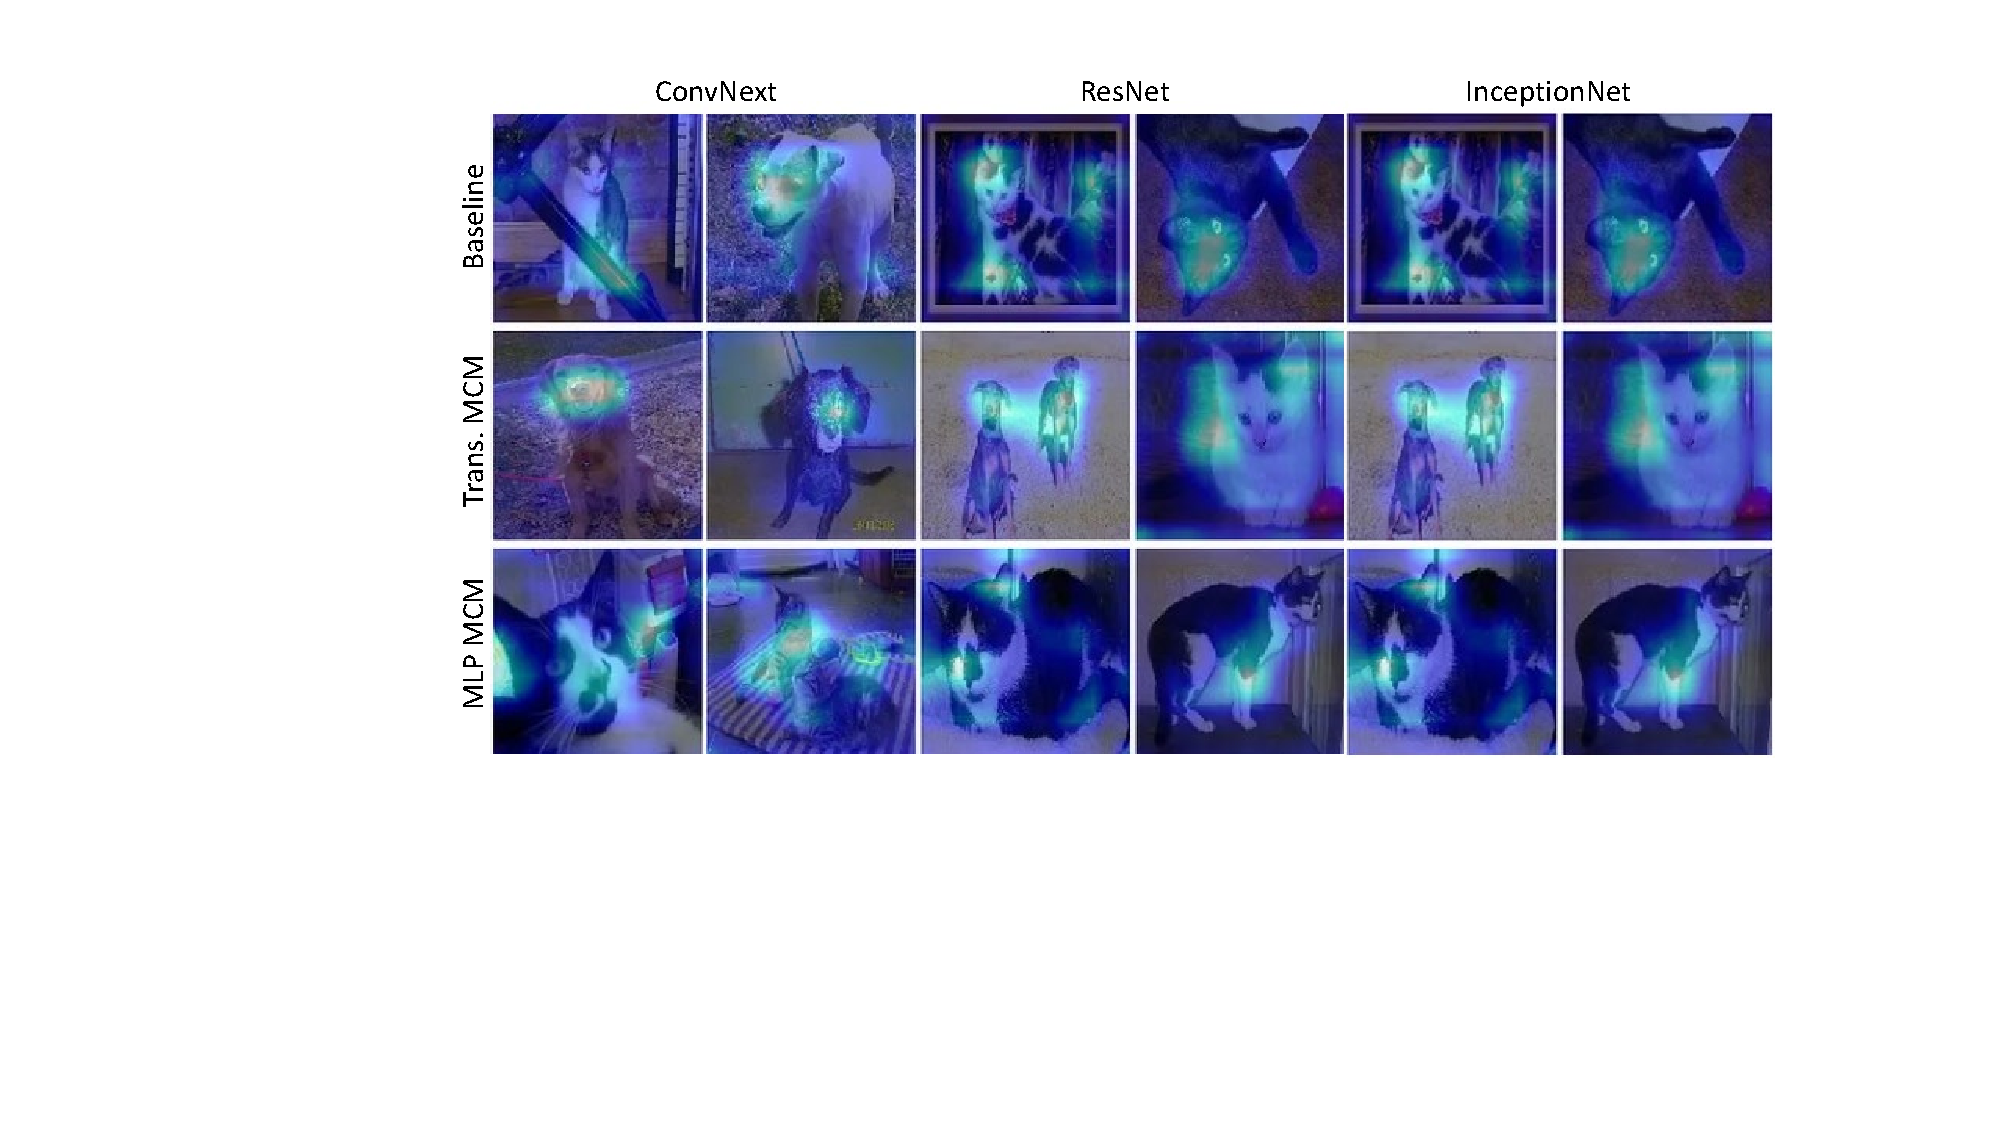
\includegraphics[width=0.5\textwidth]{figures/GrradCAM.pdf}
% 	\caption{Grad-CAM comparison.}
% 	\label{fig:GrradCAM}
% \end{figure}
% \subsection{Results and Analysis}


% \noindent\textbf{TMAM and MMAM}
% % To save additional computational complexity, the amount of calibration residual network is one.
% For Transformer-based MAM (TMAM), the transformer blocks for cross-scale relation modeling is two, which is found to be the best balancing performance and speed.
% For MLP-based MAM, the additional computations only stem from the two MLP layers.


% \noindent\textbf{Application on Other Tasks.}
% The proposed MAM aims at enhancing multi-scale relation modeling.
% We expect that future works apply the lightweight plugins in other models to improve the performance of other detection tasks.

%%%%%%%%%%% CROSS-API %%%%%%%%%
\begin{table*}
\begin{center}
   \caption{Cross-API performance. Models trained on the Megvii set are tested on the Tencent set. Since different APIs determine levels according to their own criteria, we only evaluate TP in the test.}
   \label{table:cross_tencent}
\begin{tabular}{c|c|ccc|ccc|ccc|ccc|ccc}
\hline 
&\multirow{2}{*}{Network}&\multicolumn{3}{c}{Eye Enlarging} &\multicolumn{3}{c}{Face Lifting}&\multicolumn{3}{c}{Smoothing} &\multicolumn{3}{c}{Whitening} &\multicolumn{3}{c}{Sum}\\\
& & TP & TN & AC & TP & TN & AC & TP & TN & AC & TP & TN & AC & TP & TN & AC
\\
\hline  \hline
\multirow{3}{*}{\rotatebox{90}{Direct}} & DenseNet121-MAM &.783 &.903 &.698 &.376 &.962 &.668 &.086 &.989 &.638 &.041 &.974 &.621 &.196 &.892 &.185\\
& InceptionV3-MAM &.619 &.961 &.673 &.112 &.976 &.629 &.017 &.988 &.632 &.115 &.906 &.587 &.119 &.895 &.150\\
& ResNet50-MAM &.559 &.956 &.665 &.114 &.974 &.628 &.005 &.997 &.634 &.048 &.963 &.616 &.100 &.930 &.150\\
\hline  \hline
\multirow{3}{*}{\rotatebox{90}{Finetune}} & DenseNet121-MAM &.918 &.995 &.938 &.930 &.987 &.915 &.999 &.951 &.968 &.911 &.994 &.856 &.907 &.953 &.722\\
& InceptionV3-MAM &.907 &.942 &.840 &.642 &.989 &.761 &.997 &.935 &.958 &.950 &.973 &.835 &.803 &.900 &.530\\
& ResNet50-MAM &.670 &.998 &.840 &.413 &.985 &.709 &.999 &.884 &.926 &.784 &.998 &.830 &.601 &.914 &.477\\
\hline  \hline
\multirow{3}{*}{\rotatebox{90}{Full}} & DenseNet121-MAM &.940 &.994 &.947 &.899 &.998 &.927 &.997 &.987 &.991 &.984 &.983 &.893 &.931 &.976 &.788\\
& InceptionV3-MAM &.868 &.995 &.913 &.755 &.980 &.791 &.999 &.952 &.970 &.942 &.996 &.905 &.835 &.951 &.651\\
& ResNet50-MAM &.892 &.974 &.879 &.825 &.970 &.819 &.999 &.973 &.983 &.981 &.981 &.894 &.883 &.936 &.650\\
\hline 
\hline
\end{tabular}
\end{center}
\end{table*}

%%%%%%%%%%%%% ABLATION %%%%%%%%%%%%%%%%%%%%
\begin{table}[!t]
% \renewcommand{\arraystretch}{1.2}
\centering
  % \resizebox{0.48\textwidth}{!}{
  \caption{Ablation studies and parameter settings. Network: DenseNet121-MAM. Task: in-API testing on Megvii.}
\label{table_ablation}
\begin{tabular}{c|ccc}
\hline
\multirow{2}{*}{Test} &\multicolumn{3}{c}{Sum} \\
  \cline{2-4}  & TP & TN & AC \\

\hline
\hline
% using single-labeled GT & .423  & .641 & .103\\
Smaller clustering rate: $r=[\frac{1}{32},\frac{1}{8},\frac{1}{2},1]$ & .397 & .708 & .192 \\
Larger clustering rate: $r=[\frac{1}{128},\frac{1}{32},\frac{1}{8},\frac{1}{2}]$ & .355 & .842 & .230 \\
More trans. layers within MAM: $d=4$ & .473 & .902 & .347\\
Less trans. layers within MAM: $d=1$ &.425&\textbf{.919}&.331\\
without data cleaning & .342 & .877 & .257\\
without data augmentation & .279 & .854 & .175\\
\textbf{Default Setting}  & \textbf{.519}  & .895 & \textbf{.366} \\
\hline
\end{tabular}
% }
\end{table}

%%%%%%%%%%%%% ALIBABA PERFORMANCE %%%%%%%%%%%%%%%%%%%%
\begin{table}
\begin{center}
   \caption{Cross-API performance. Models trained on the Megvii set are tested on the Alibaba set (containing only single-operated images) directly, without any finetuning.}
   \label{table:cross_alibaba}
\begin{tabular}{c|c|c|c|c|c}
\hline 
\multirow{2}{*}{Network}&{Eye} &{Face}&{Smo.} &{White.} &{Sum}\\\
& TP & TP & TP &  TP & TP
\\
\hline  \hline
InceptionV3~\cite{inceptionv2}&.430&.467&.633&.605&.534 \\
ResNet50~\cite{ResNetv2}&.513&.449&.373&.496&.458\\
ConvNextV1~\cite{ConvNext}&.721&.436&.557&.602&.579 \\
DenseNet121~\cite{DenseNet}&.526&.553&.662&.636&.594 \\
EfficientNet~\cite{tan2019efficientnet}&.326&.169&.771&.380&.412 \\
% \hline 
% \hline
% ViT~\cite{dai2021coatnet} \\
% Swin-T~\cite{Swin} &.562&1.&.562&.570&1.&.570&.568&1.&.568&.567&1.&.567&.186&1.&.186\\
\hline 
\hline
\textbf{InceptionV3-MAM}&.440&.368&.795&.555&.539~\li{+.005}\\
\textbf{ResNet50-MAM}&.390&.302&.668&.505&.466~\li{+.008}\\
\textbf{DenseNet121-MAM}&.519&.548&.861&.501&.607~\li{+.013} \\
\hline 
\hline
\end{tabular}
\end{center}
\end{table}

\subsection{In-API Performances}
% ``in-API" denotes the test where users train and test models both on the same subset \texttt{A}.
We show the performance on the Megvii set in Table~\ref{table:full_experiment_megvii} and that on the Tencent set in Table~\ref{table:cross_tencent}. We also conduct ablation studies on the in-API Megvii set test in Table~\ref{table_ablation}.
We find that CNN architectures can perform generally better in our task compared to the transformer and hybrid counterparts.
For example, the overall TP for InceptionNet and DenseNet are above 0.5, which leads by a noticeable margin.
Yet we see that for these models as well as many of the rest, the detection accuracies on geometric operations are lacking.
We introduce MAM into respectively InceptionNet, ResNet and DenseNet, and find that the overall performance w.r.t both TP and AC increased a lot, and the detection results on the geometric operations are significantly improved.
% For artifact discovery, CNNs are already proven excellent in pattern recognition.
% For joint analysis on items in multiple scales, 
% we find that existing classification architectures usually carry implicit multi-granularity learning.
Our view is that most CNN backbones have their classifiers operated on the lowest-resolutioned representations, e.g., $7\times~7$, which might lack multi-granularity modeling.
Though the residual connection~\cite{ResNetv2} and inception-like modules~\cite{inceptionv2} can combine features of different receptive fields, the operations are on the basis of whole feature maps, therefore retaining spatial redundancy and lacking focus on what to attend. 
% enjoys explicit hierarchical representation learning where the shallow layers are believed to generally gather information from smaller receptive fields while the later layers grasp semantic meanings.
% Though CrossViT~\cite{chen2021crossvit} and Conformer~\cite{conformer} also consider explicit multi-granularity modeling with the help of the Transformer architecture ,
% For example, CrossViT~\cite{chen2021crossvit} and MUSIQ~\cite{MUSIQ} are two similar ways of feeding Transformer with multi-resolutioned images.
% Conformer~\cite{conformer} use two-streamed networks combining convolutional operations and self-attention.
% these networks are usually computationally heavy and, more importantly, marginal in performance increase compared to the CNN counterparts (see Section~\ref{section:experiment}).
% Transformers can mitigate this issue with self-attention.
% Recently some works apply CNN blocks in Transformers to enhance local representation learning.
% However, they usually require heavy computation and still do not provide satisfactory, or even worse results in our task. 
% MUSIQ~\cite{MUSIQ} also introduce multi-scality to capture information at different granularities, they only input images at different resolutions into the Transformer architecture.
% In comparison, the proposed MAM can jointly utilize the benefit of CNN backbone and redundancy reduction.
% Besides, the false alarms are also decreased.
In Table~\ref{table:multi_process_megvii}, we further report the TPs on the comparatively heavy retouched, i.e., triple- and quad- operated images.
% \needattention{We include more analysis towards the effect of MAM in the supplementary materialary material.}
For all four operations, after adding the MAM on different backbones, the TPs are mostly improved.
% We also find that different models can have specializations on the detection of different types. For example, the overall TPs of InceptionNet-MAM for non-geometric operations both exceed 0.92, while that of Densenet-MAM for geometric operations leads by over five percent.
% Also, we find that AC is usually 10\% lower than TP.
% Besides the extra challenge of distinguishing different levels, for some images, the 60-leveled operations might already give saturated results, resulting in little difference with that of the 90-leveled ones.
% However, AC is still an important indicator if we need to forbidden retouching according to levels, and the experiments show that the averaged ACs of models with MAM are higher than 0.3 and those without MAM below 0.3.

\noindent\textbf{Ablation Studies.}
We also study the effect of data cleaning and network designs of MAM.
Notice that in ``w/o data cleaning", we exclude invalid data in the test set, meaning that there will be more but noisier data in the training stage.
In ``w/o data augmentation", we train the models on the unaugmented images and test them on the augmented images.
The studies show that the existence of noisy data and excessive image details will mislead the models from learning faulty representations, and the proper setting of $r$ and $l$ also affects the overall performance.

\subsection{Cross-API Performances}
% ``Cross-API" denotes the test where users train models based on Subset \texttt{A} and validate them on Subset \texttt{B}.
% It simulates that users train models on existing retouched images and deploy them in real-world environments. 
Due to that AC is strict in definition which does not consider API discrepancies, we report the TP values in each test.
% The discrepancies between different APIs are showcased in Fig.~\ref{fig:difference}.
% \noindent\textbf{cross-API Detection Accuracy.}
Provided with the models trained on the Megvii set, we empirically find that they can be directly tested on the Alibaba set, while it requires some finetuning to be well-roundedly tested on the Tencent set.
% Fig.~\ref{fig:API_diff} show exampled groups of retouched images with the same setting, where the smoothing can be performed on different regions and whitening renders different face colors.
% \noindent\textbf{Finetuning on Larger-Gaped Subsets.}
% We find that there might be large visual gaps within images generated by different APIs.
% For example, the detection models trained on the Megvii dataset can only detect eye-enlarging and face-lifting, but largely fail to detect the rest two types.
% In order to mitigate the gaps in the retouching protocol,
% in real-world application, we can collect a few retouched images from the new platform and finetune the detection models to cater to the new protocols and pursur better cross-API performance.
We finetune the models on the Tencent set for 10,000 iterations (accounting for around 15\% of all images) and report the performances together in Table~\ref{table:cross_tencent}. 
For reference, we also train models from scratch till convergence on the Tencent set, and report the in-API performance in the same table.
We find that the short finetuning is effective enough for models to adjust to the new protocols of the new platform.
The performance of training on the Tencent set and testing on the Megvii set yields similar results.
We omit it for space limit.
% \noindent\textbf{Direct Application on Smaller-Gaped Subsets.}
% We also find that finetuning is not always needed if the API gaps are small.
% For example, models trained on the Megvii set can be directly applied to infer the images from the Alibaba dataset with acceptable performance drop.
Table~\ref{table:cross_alibaba} reports the performances by direct cross-API application on the Alibaba set.
% We report the TPs since there only exists single-operated images.
The results show that both the baseline networks and those with MAM have performance generalization. 
While the performances of models with MAM on in-API tests are better, it is also the case for cross-API tests w.r.t. overall TPs.


% \noindent\textbf{Heatmap Visualization.}
% In Fig.~\ref{image_heatmap}, we measure the discriminative capability of the multi-view representations using heatmap visualization. We arbitrarily select ten real news and ten fake news. 
% % Each sub-figure therefore shows the correlation pattern between inter-class news and intra-class news provided with different views of representations. 
% From the figures, the bootstrapped representation shows strong discriminative capability where intra-class similarity and inter-class difference are both noticeable. 

% \begin{table}[!t]
% % \renewcommand{\arraystretch}{1.2}
%     \setlength{\tabcolsep}{1.5mm}
% 	\caption{\textbf{Computational overhead of MAMs on ResNet50.}}
% 	\label{table_complexity}
% 	\begin{center}
% 	\begin{tabular}{c|c|c|c}
% 		\hline
% 		{Method} & {Params} & {Memory}  & {FLOPs}\\
%         \hline
%         \hline
%         ResNet50 & 23.6M & 73MB  & 22.3G \\
%         ResNet50+MAM & 68.8M & 172MB  & 44.7G \\
%         \hline
%         \hline
%          InceptionV3 & 6.0M & 39MB  & 8.3G \\
%         InceptionV3 V1+MAM & 74.5M & 333.2MB  & 52.7G\\
%         \hline
%         \hline
%         Conformer & 81.8M & 392MB  & 118.9G \\
%         Swin-T & 30.5M & 122.8MB  & 17.4G \\
%         CoAtNet & 5.0M & 22.18MB  & 13.9G \\
%         CMT & 44.0M & 310MB & 36.1G \\
% 		\hline
% 	\end{tabular}
% 	\end{center}
% \end{table}

% \noindent\textbf{Computational Overhead.}
% The computational complexity study in Table~\ref{table_complexity} shows that BMR requires less trainable parameters compared to EANN and SpotFake. 
% CAFE requires amazingly low computational complexity by using simple auto-encoders and MLPs, but the performance is not good enough.


%%%%%%%%%%%%%%%%%%%%%%%%%%%%%%%%%%%
%%%%%%% begin of sec:related %%%%%%%

% \section{Related Works and Datasets}
% \label{section:related}
% \subsection{Datasets of Human Faces}
% In various social media, short video platforms, we can see a variety of people sharing their joys and sorrows. As one of the representations used for identity recognition, the face has received much attention and research by scholars.  Face-based tasks include face recognition, 3D face reconstruction, face face retouching, face expression transfer, and face generation. Researchers have proposed a series of Face datasets for different tasks, e.g. LFW (Labeled Face in the Wild), CelebA, etc. The dataset includes a variety of complex scenes and demographic features such as skin color, age, background, pose, accessories, expression, etc. 
% Besides, FFHQ (Flickr-faces-high-quality) is also a widely-known dataset which contains 70,000 PNG format high-definition face images with 1024×1024 resolution from Flickr, covering a wide range of images. 
% Previously, a number of advanced face recognition or processing datasets are built upon FFHQ, e.g., FFHQR~\cite{FFHQR}, FFHQ-UV~\cite{FFHQUV} and CelebA, e.g., CelebV-Text~\cite{CelebVText}, Celeb.

% Our proposed RetouchingFFHQ is built upon the original (non non-retouched) images from FFHQ. 
% It does not indicate that face face retouching detection tasks cannot perform on images based on CelebA.
% The higher resolution and smaller amount of FFHQ has earned our favour, and we leave extending the task on CelebA in future works.
% To ensure that the original images in FFHQ would maximally differ from their retouched versions, we also conduct tailored data cleaning as specified in Section~\ref{sec:data_clean}.

% \subsection{Face Retouching}
% In the past decades, with the rise of social networking, retouching on the face images has become a common practice. Researchers have shown the impact of face face retouching in the performance degradation of face recognition algorithms, which shows the necessity of detection


% \noindent\textbf{Datasets.} 
% Bharati et al. proposed one of the largest datasets, the ND-IIITD database, covering seven presets of retouching by gender. The dataset contains 325 original images of UND-B identities, 2600 original and 2275 retouched face images. The authors also created a Celebrity dataset with 330 images belonging to 165 celebrities from the Internet. Each has an original and a retouched image. Later, Bharati et al. developed a demography-based retouched face dataset, Multi-Demographic Retouched Faces (MDRF), containing subjects belonging to three ethnicities, Indian, Chinese, and Caucasian with 3600 images in total.

% \subsection{DeepFake Detection}

% A number of methods have been proposed to detect deepfake images. Early works use hand-crafted features to seek for the artifacts in forged faces, such as steganalysis features. The physiological signs are exploited to detect the inconsistency of the face movement or the environment. Several specific representations (eg., eye blinking, head poses, optical flow, emotion, neuron behaviors, mouth movement, heart rate) are used to aid detection. Some approaches considered noises from generative models. Yu N et al. detect GAN fingerprints, while Guarnera L et al. consider the convolutional traces in the images. More recent works focus on the frequency domain, using DCT , local frequency or SRM. To take advantage of subtle artifacts, Gu Q et al. first perform fine-grained decomposition in the frequency domain, and propose a progressive enhancement learning network to exploit the combined fine-grained frequency components and RGB image. Other works such as Face X-ray or PCL also bring different perspectives to the deepfake detection task. 


% \noindent\textbf{Datasets.}
% Early works such as UADFV and DeepFake-TIMIT are small datasets. 
% FaceForensics++ is the first large-scale face forensic dataset that consisted of 4, 000 fake videos manipulated by four methods (i.e., DeepFakes, Face2Face, FaceSwap, and NeuralTextures), as well as 1,000 real videos from YouTube. Afterward, Google contributed DeepFake Detection [13] dataset with 3, 431 real and fake videos from 28 actors. 
% More recently, larger Deepfake datasets are released, such as DFDC consisting of over 120,000 videos and WildDeepfake dataset consisting of over 7000 images.

% \noindent\textbf{\ying{Difference with Fine-grained Retouching Detection.}}
% Although both DeepFake detection and retouching detection originate from face forgery detection, the noticeable differences can be summarized as follows. First, the Deepfake image originates from two different images and a blending operation is required. The area of the modification is large, and both images always contain inconsistent sensor or compression noise. In comparison, the traces of manipulation that can be detected from retouched images are more subtle. Second, Deepfake detection is mainly a binary problem, unlike beauty detection, which may include degree detection.


%%%%%%%%%% begin of sec:conclusion
\section{Conclusion}
\label{section:conclusion}
In this paper, we introduce a large-scale and fine-grained face retouching dataset, RetouchingFFHQ, which enables more effective research in the field of face retouching detection. By considering different retouching types and levels, we extend the binary detection problem into a fine-grained, multi-retouching type, and multi-retouching level estimation problem. To enhance feature extraction, we propose a Multi-granularity Attention Module (MAM) as a plugin for CNN backbones. Extensive experiments using different baselines as well as our proposed method on RetouchingFFHQ show decent performance on face retouching detection.

% \noindent\textbf{Future Works.}
% % Though we filtered out OOD examples, there can still exist images with slight makeups that escaped the cleaning stage.
% % Besides, we are not able to conduct quantified retouching detection on images from popular short-video platforms such as TikTok, due to the lack of relevant API so far.
% Given the fine-grained prediction result, it would be of great value to further estimate possible original faces of the retouched images in livestreams, therefore offering references for users' subjective judgement.

\bibliographystyle{ACM-Reference-Format}
\balance
\bibliography{sample-sigconf}

\end{document}
\endinput
%%
%% End of file `sample-sigconf.tex'.
